%%%%%%%%%%%%%%%%%%%%%%%%%%%
% PREAMBOLO DEL DOCUMENTO %
%%%%%%%%%%%%%%%%%%%%%%%%%%%

\begin{filecontents*}[overwrite]{\jobname.xmpdata}
    \Title{Predizione di vulnerabilità software tramite machine learning}
    \Author{Moscato Gabriele}
    \Language{it}
    \Subject{Questo studio si pone l’obiettivo di indagare sulle cause, sull’impatto economico e sociale causato dalle vulnerabilità software. Lo studio si focalizza principalmente su come e in che modo l’uso di modelli di machine learning posso essere utili per evitare e individuare vulnerabilità software.Durante il mio lavoro di tesi ho analizzato alcuni studi svolti in passato in questo ambito ele prestazioni ottenute da quest’ultimi, sulla base di questi studi ho sviluppato un modello di predizione basato su machine learning capace di predirre la presenza di vulnerabilità software per applicazioni Java, il mio studio si conclude analizzando le prestazioni ottenute dal predittore.}
\end{filecontents*}


\documentclass[a4paper,11pt,oneside,top=3cm,bottom=3cm,left=3.5cm,right=3.5cm,openright,reqno,table]{book}

% openany - fa iniziare i capitoli direttamente nella pagina successiva
% openright - fa iniziare i capitoli nella prima pagina destra disponibile 
% fleqn  - allinea le formule a sinistra anzichè centrarle
% leqno - dispone la numerazione delle formule sulla sinistra o destra
% reqno - dispone la numerazione delle formule sulla destra
%
\usepackage{packages}
\usepackage{natbib}
% Per non appesantire troppo questo file
% quasi tutti i pacchetti usati sono salvati in packages.sty
%
\linespread{1.5}
% Per avere la parola BOZZA scritta su tutte le pagine

% funziona solo in modalità PS
% Invece per i PDF ho risolto così:
% pdftk tesi.pdf background bozza.pdf output tesi_bozza.pdf
%
%%%%%%%%%%%%%%%%%%%%%%%%%%%%%%%%%
%   DOCUMENTO VERO E PROPRIO    %
%%%%%%%%%%%%%%%%%%%%%%%%%%%%%%%%%
\begin{document}
% FRONTESPIZIO %
\begin{titlepage}
\changepage{}{}{}{-7.5 mm}{}{}{}{}{}
% parametri per cambiare le dimensioni di una singola pagina in ordine:
% {textheight}{textwidth}{evensidemargin}{oddsidemargin}{columnsep}
% {topmargin}{headheight}{headsep}{footskip}
% se voglio centrare la pagina devo mettere bindingoffset/2
% i primi 5 parametri posso usarli con \changetext


\begin{center}

\includegraphics [width=.15\columnwidth, angle=0]{unisa}\\ % height
\vspace{0.5cm}
{\LARGE \scshape Università degli Studi di Salerno}\\
\vspace{0.5cm}
{\Large Dipartimento di Informatica}\\
\vspace{0.1cm}
{\large Corso di Laurea Triennale in Informatica}\\
\vspace{1.5cm}
{\Large \scshape Tesi di Laurea} \\
\vspace{4cm}
{\Huge \bfseries Predizione di vulnerabilità software tramite machine learning} \\
\vspace{5cm}

\begin{minipage}[t]{7cm}
\flushleft
\textsc{Relatore}

Prof. \textbf{Fabio Palomba} \\
{\small Università degli studi di Salerno} \\[0.25cm]
\end{minipage}
\hfill
\begin{minipage}[t]{7cm}
\flushright
\textsc{Candidato}

\textbf{Gabriele Moscato} \\
Matricola: 0512108099
\end{minipage}

\vspace{3cm}

%& & \\
%& Candidato & \\
%& \textbf{Fabiano Pecorelli} & \\
{\small Anno Accademico 2021-2022} %\\
%
%
\begin{comment}
\begin{table}[!h]
\centering
\begin{tabular}{c c c} %p{5cm}c
& Tesi di laurea & \\
& \textbf{Fabiano Pecorelli} & \\
& & \\[0.25cm]
Relatore \\
prof. \textbf{Andrea De Lucia} \\
{\small Università degli studi di Salerno} & & {\small Provincia di Salerno}\\
& & \\[0.5cm]
& {\small A.A. 2015-2016} & \\
\end{tabular}
\end{table}
\end{comment}
%
%
\end{center}

\end{titlepage}
%


\frontmatter
% quello che segue è in numerazione romana e i capitoli non verranno numerati
% se non si vuole che compaia il numero di pagina basta usare il comando:
%\nonumber

% RINGRAZIAMENTI %
\begin{titlepage}

\nonumber
\null \vspace {\stretch{1}}
	\begin{flushright}
%	\begin{verse}
\textit{"Ascolta quel che insegna la sapienza, cerca di capire la sua lezione. Ricerca la conoscenza e desidera la saggezza, come si desidera l’argento o si va in cerca di tesori"} (La Bibbia).\\[5mm]
%	\end{verse}
	\end{flushright}
	
\end{titlepage}
% SOMMARIO %
\cleardoublepage
\selectlanguage{italian}
\begin{abstract}
Questo studio si pone l'obiettivo di indagare sulle cause, sull'impatto economico e sociale  causato dalle vulnerabilità software. 
Lo studio si focalizza principalmente su come e in che modo l'uso di modelli di machine learning posso essere utili per evitare e individuare vulnerabilità software. \newline
Durante il mio lavoro di tesi ho analizzato alcuni studi svolti in passato in questo ambito e le prestazioni ottenute da quest'ultimi, sulla base di questi studi ho sviluppato un modello di predizione basato su machine learning capace di predirre la presenza di vulnerabilità software per applicazioni Java, il mio studio si conclude analizzando le prestazioni ottenute dal predittore. \\[1cm]
\end{abstract} 
% INDICI %
\phantomsection
\addcontentsline{toc}{chapter}{Indice}
\tableofcontents
% Il simbolo * serve per evitare che comapaia nell'indice
\clearpage
%\listoffigures
%\clearpage
%\listoftables
% GLOSSARIO
%\cleardoublepage
\phantomsection
\addcontentsline{toc}{chapter}{Glossario}
% per inserire l'elenco dei simboli e degli acronimi nell'indice
\printglossary
% Per stampare il glossario
% per aggiornarlo si deve eseguire da terminale:
% makeindex -s myDoc.ist -t myDoc.alg -o myDoc.acr myDoc.acn
% per inserire una voce nell'elenco:
% \newglossaryentry{voce_etichetta}{name={voce}, description={descrizione}}
% se non compare direttamente nel testo va inizializzata con:
% \glsadd{voce_etichetta}
% oppure se viene richiamata all'interno del testo:
% \gls{voce_etichetta}
% SIMBOLI E NOTAZIONI %
\cleardoublepage
\phantomsection
\addcontentsline{toc}{chapter}{Elenco delle figure}
% per inserire l'elenco dei simboli e degli acronimi nell'indice
%\printglossary[type=\acronymtype,title=Elenco delle figure]
% Per stampare l'elenco dei simboli
\listoffigures
\cleardoublepage
\phantomsection
\addcontentsline{toc}{chapter}{Elenco delle tabelle}
% per inserire l'elenco dei simboli e degli acronimi nell'indice
%\printglossary[type=\acronymtype,title=Elenco delle figure]
% Per stampare l'elenco dei simboli
\listoftables
% per aggiornarlo si deve eseguire da terminale:
% makeindex -s myDoc.ist -t myDoc.glg -o myDoc.gls myDoc.glo
% per inserire una voce nell'elenco:
% \newglossaryentry{voce_etichetta}{name={voce}, description={descrizione}}
% se non compare direttamente nel testo va inizializzata con:
% \glsadd{voce_etichetta}
% oppure se viene richiamata all'interno del testo:
% \gls{voce_etichetta}

\mainmatter
% quello che segue sarà in numerazione araba e i capitoli verranno numerati
%\part{Studio iniziale}
% CAPITOLI
\phantomsection
%\addcontentsline{toc}{chapter}{Introduzione}
\chapter{Introduzione}
\markboth{Introduzione}{}
% [titolo ridotto se non ci dovesse stare] {titolo completo}

\section{Contesto applicativo} 
Con l'espansione e la crescita della digitalizzazione in tutti gli ambiti della nostra società, si è verificato un aumento significativo di fenomeni criminali in ambito digitale, la sicurezza informatica nasce con il proposito di contrastare e annullare questa tipologia di criminalità.
La sicurezza informatica non ha come scopo solo quello di evitare attacchi informatici ma anche quello di offrire software o dispositivi capaci di essere robusti e affidabili, evitando che questi possano essere compromessi.
\newline La crescita dello spazio cibernetico ovvero l'interconnessione delle infrastrutture informatiche \citep{dei2013quadro} ha reso i sistemi informatici su cui si fonda più vulnerabili a possibili manipolazioni, con l'avanzare degli anni tutto ciò sta causando una crescita graduale degli attacchi informatici nel mondo, i quali stanno diventano sempre più frequenti e complessi coinvolgendo sempre più tipologie di vittime e causando danni economici sempre maggiori.
Lo sviluppo della criminalità informatica è dovuto anche al modo in cui possono operare gli hacker, infatti lo spazio cibernetico consente loro di poter compiere un attacco i qualsiasi posizione fisica colpendo in modo istantaneo l'obiettivo e in modo quasi del tutto anonimo. \newline 
Internet è nato come un' \textit{ungoverned space} ovvero non regolamentato da autorità politiche o internazionali \citep{baldoni2015futuro}, tuttavia a causa di una maggiore pressione in ambito di sicurezza pubblica e a causa di attacchi che in più situazioni hanno coinvolto enti nazionali, diverse nazioni si stanno mobilitando per cercare di offrire più sicurezza online ai propri cittadini.
\begin{figure}[!htb]
    \centering
    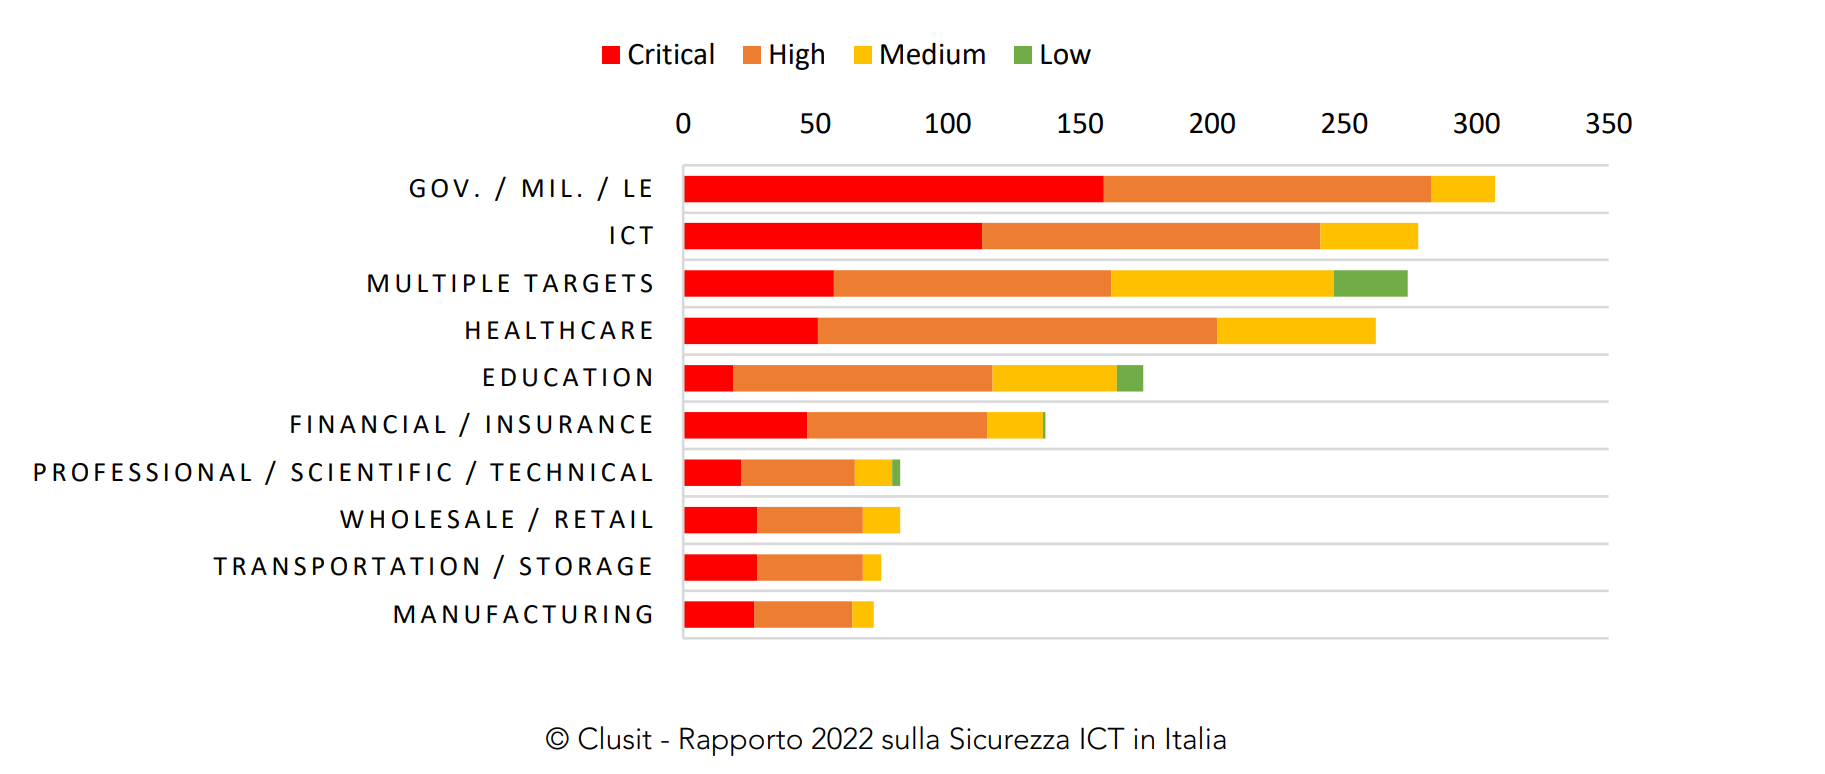
\includegraphics[scale=0.7]{../figure/target.png}
    \caption{Top 10 vittime 2021 in Italia}
    \label{fig:top10vittime}
\end{figure}
In questo senso uno degli attacchi hacker che ha fatto molto discutere in Italia è avvenuto il 30 luglio 2021 al CED (centro elaborazione dati) della regione Lazio \citep{LazioAttack}, l'attacco ha mandato in tilt i servizi di privati e aziende, coinvolgendo anche il sistema sanitario della regione dedicato alla vaccinazione contro il COVID-19, gli effetti sono stati molto gravi provocando un mese di interruzione di alcuni servizi tra cui alcuni urbanistici, ma coinvolgendo sopratutto servizi sanitari online. L'attacco informatico subito è definito \textit{ransomware} \citep{Ransomware} questa tipologia di attacco si diffonde attraverso un programma dannoso (malware), che ha come scopo quello di bloccare l'accesso ai contenuti presenti sul dispositivo infetto, per poi richiedere un riscatto per renderli di nuovo accessibili, nel caso della regione Lazio dalle ricostruzioni l'infezione è partita da un computer di un dipendente, dal quale i criminali sono riusciti ad accedere ai servizi di un dipendente con privilegi di admin, tramite quest'ultimo sono riusciti ad accedere ai dati per poi criptarli. 
\newline Attacchi come quello avvenuto alla regione Lazio mostrano come queste attività criminali possono incidere notevolmente sulla sicurezza delle istituzioni e dei cittadini, questi eventi stanno portando gli enti nazionali e internazionali a mobilitarsi per poter prevenire e combattere questa tipologia di criminalità.
\begin{figure}[!htb]
    \centering
    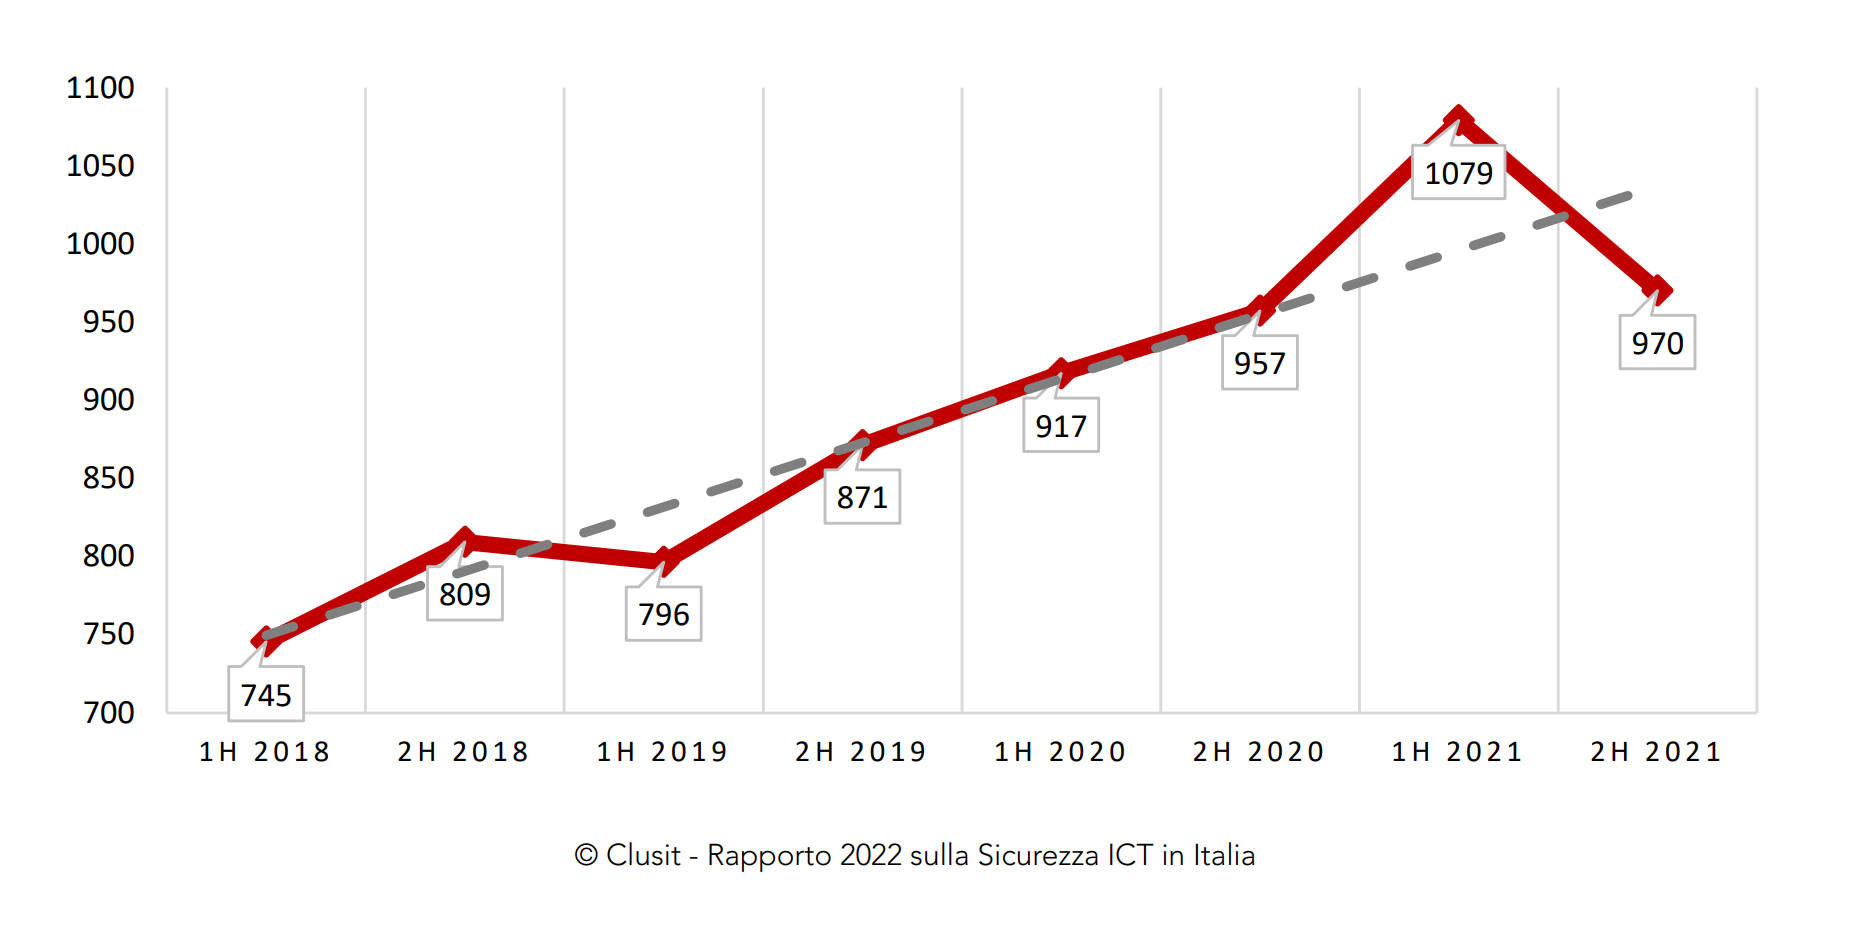
\includegraphics[scale=0.8]{../figure/attacchi per semestre.png}
    \caption{Attacchi per semestre dal 2018}
    \label{fig:attacchiPerSemetre}
\end{figure}
\newline In Italia, negli ultimi anni, il tema della sicurezza informatica sta assumendo una posizione sempre più rilevante, uno degli interventi più importanti è il decreto-legge n. 105 del 2019 il quale è nato con lo scopo di garantire un elevato livello di sicurezza delle reti e dei sistemi informatici delle pubbliche amministrazioni, dei servizi informatici e degli enti e operatori nazionali \cite{SicurezzaCibernetica}. Attualmente la sicurezza cibernetica è uno dei progetti principali finanziati dal \textit{PNRR} (Piano nazionale di ripresa e resilienza) \citep{italiano2021piano}, a cui sono destinati 620 milioni di euro per il rafforzamento delle infrastrutture legate alla protezione cibernetica in Italia. 
Anche l'Europa attraverso la Commissione europea sta spingendo gli Stati membri a rafforzare le proprie difese informatiche, in particolare nel 2016 è stata introdotta la prima misura legislativa per tutta l'Europa in ambito di sicurezza cibernetica, la \textit{Direttiva NIS} \citep{nis}, che poi, a fronte di una notevole accelerazione della digitalizzazione causata dalla crisi COVID-19, la Commissione europea nel dicembre del 2020 ha proposto la direttiva NIS riveduta (\textit{NIS2})\citep{nis2}.
\newline Con il trascorrere degli anni il numero degli attacchi informatici sta aumentando, con essa sta crescendo la gravità degli attacchi e la loro complessità, aumentando i costi ad esso associati. Il \textbf{Clusit} (Associazione Italiana per la Sicurezza Informatica) \citep{clusit} periodicamente rilascia report sulla situazione italiana in ambito di sicurezza informatica, nell'ultimo rapporto avvenuto a marzo del 2022 \citep{clusitReport} il Clusit ha riportato che nel 2021 il numero di attacchi informatici nel mondo ha registrato un aumento di circa 10\% rispetto al 2020, un dato molto preoccupante è l'aumento dell'impatto degli attacchi infatti il 79\% di questi ha avuto un impatto elevato. Un importante analisi è stata condotta per il territorio italiano che ci permette di analizzare la situazione in Italia, dalla figura~\ref{fig:attacchiPerSemetre} possiamo denotare come dal 2018 il numero di attacchi in Italia è cresciuto enormemente, con un picco di 1079 attacchi nel primo semestre del 2021, un dato molto importante da considerare in ambito di sicurezza informatica sono le vittime degli attacchi, infatti gran parte di queste, come si evince dalla figura \ref{fig:top10vittime}, sono enti nazionali e governativi, rispetto al 2020 però le categorie che hanno avuto un aumento considerevole di attacchi nell'ultimo anno sono Transportation/Storage con un aumento del 93,3\% e la categoria di News/Multimedia con un aumento del 60,5\%. \newline
\begin{figure}
    \centering
    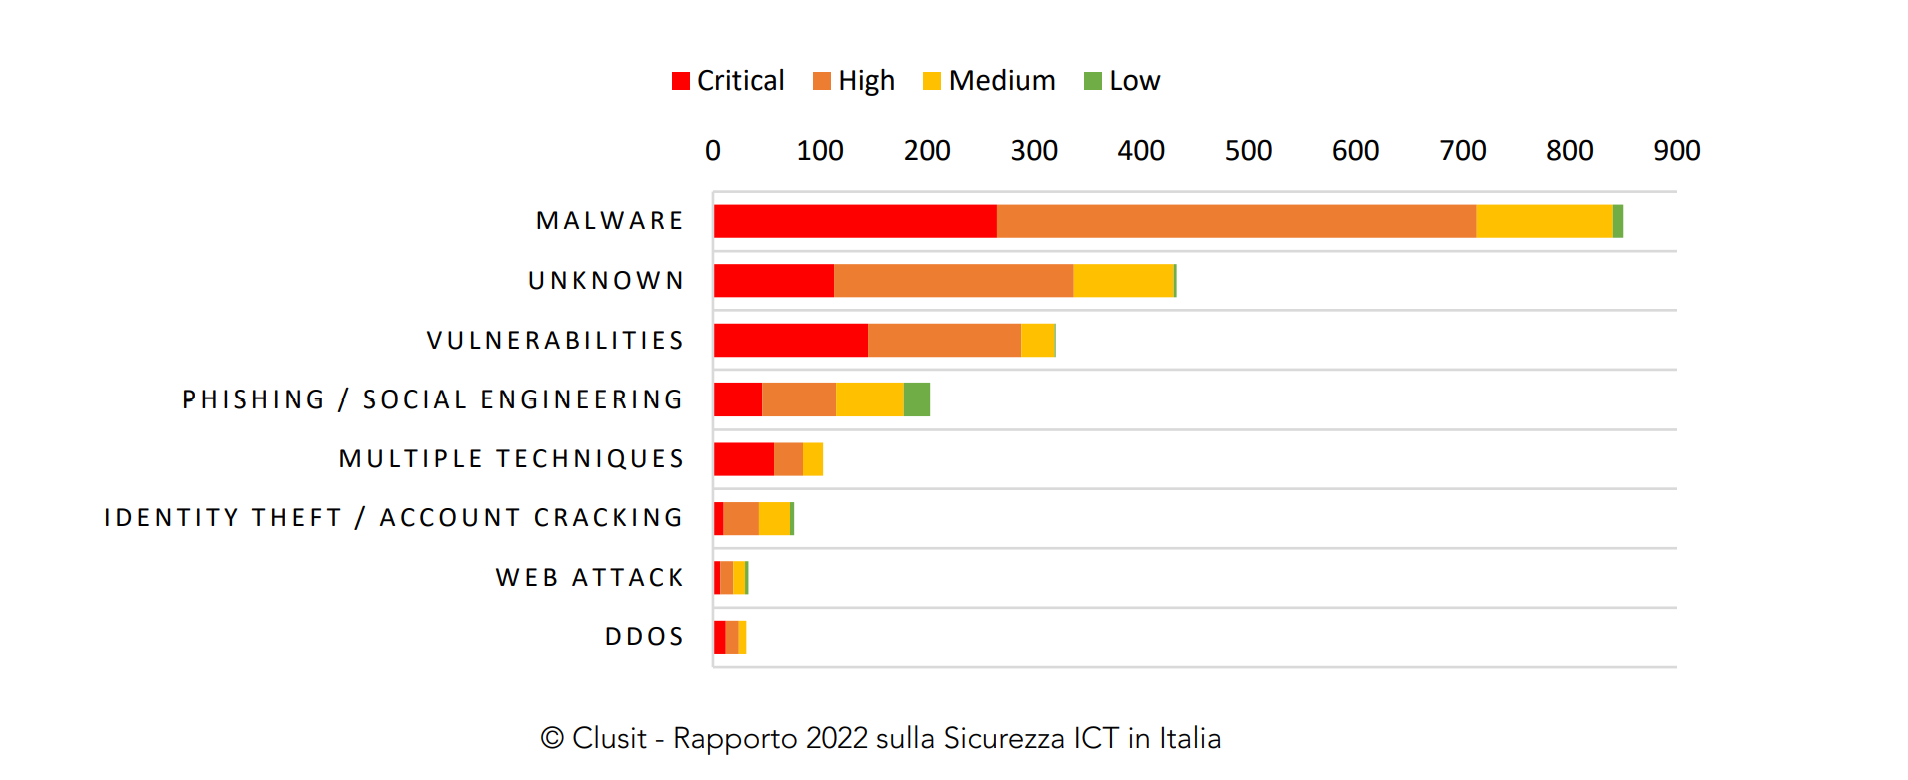
\includegraphics[scale=0.8]{../figure/clusit attacchi.png}
    \caption{Tecniche di attacco 2021}
    \label{fig:tecnicheDiAttacco}
\end{figure}
\begin{figure}
    \centering
    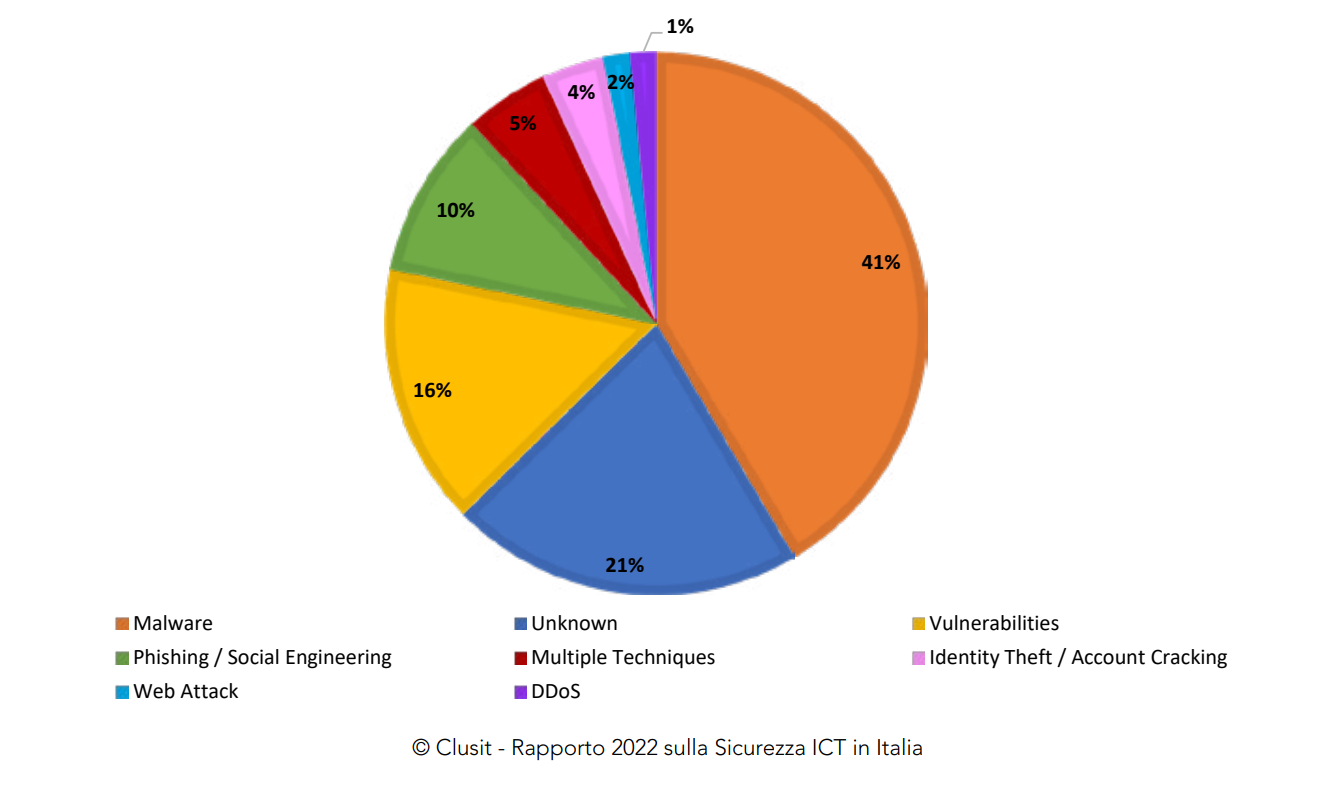
\includegraphics[scale=0.9]{../figure/tipologiaAttacchiTorta.png}
    \caption{Distribuzione tecniche di attacco 2021}
    \label{fig:tecnicheDiAttaccoTorta}
\end{figure}
Uno dei dati più interessanti anche in termini di prevenzione è il modo attraverso cui gli hacker riescono ad effettuare un attacco informatico, figura \ref{fig:tecnicheDiAttacco} e figura \ref{fig:tecnicheDiAttaccoTorta} ci mostrano quali sono e in che modo sono distribuiti, da quanto possiamo notare il metodo più diffuso sono i malware con una percentuale del 41\%, mentre il 21\% è sconosciuto e il 16\% degli attacchi avviene sfruttando vulnerabilità, inoltre confrontando i dati con l'anno precedente notiamo un notevole aumento di attacchi avvenuti sfruttando vulnerabilità con un aumento del 60\% di quest'ultimi, mentre i malware hanno registrato un aumento del 9.7\%, oltre a questi dati notiamo anche un incremento dell'impatto di quest'ultimi, anche in questo caso le vulnerabilità hanno registrato un aumento soprattutto di attacchi critici e alti.
\newline Come mostrato gli aspetti più critici della sicurezza informatica sono lato software, per questo motivo gran parte degli studi coinvolti in ambito di sicurezza si concentrano sui sistemi software.
La sicurezza di un sistema software nasce dalla sua origine, durante la definizione dei requisiti, in particolare durante questa fase sono definite le politiche di sicurezza che specificano ciò che è consentito e ciò che non è consentito dal sistema, più nel dettaglio definiscono la disponibilità del sistema e la definizione per ogni tipologia di utente di cosa può fare e a cosa può accedere e nel caso questi requisiti non vengano rispettati come il sistema deve comportarsi, in modo tale funzionare correttamente in caso di un errore o in caso di un attacco al sistema \citep{bishop2003computer}.
Questo mostra come un buon sviluppo del software può in parte contribuire con la creazione di un prodotto software sicuro da possibili attacchi informatici, sfortunatamente, tutto ciò non è sufficiente per evitare la presenza di possibili vulnerabilità software.

\section{Motivazioni e Obiettivi} %\label{1sec:scopo}
Come abbiamo visto la sicurezza informatica è uno dei problemi più rilevanti in campo informatico, che colpisce principalmente persone e istituzioni, attaccando la loro sicurezza e minando profondamente la salute e la privacy degli utenti. Quindi combattere la diffusione di attacchi informatici non solo ci permette di contrastare organizzazioni criminali e truffe, ma anche a salvaguardare la sicurezza nazionale, internazionale e dei singoli cittadini, la lotta contro la criminalità informatica ci permette inoltre di abbassare drasticamente i costi dovuti a danni o a truffe online.
\newline La prevenzione è uno dei metodi più efficaci per abbattere l'aumento di crimini informatici, un'infrastruttura o un prodotto software che offrono buoni sistemi di protezione contro possibili attacchi informatici sono meno vulnerabili e più affidabili, quindi sono più difficili da compromettere, lato software la realizzazione di sistemi sicuri, prevede inevitabilmente un innalzo dei costi di implementazione, sfortunatamente a causa di budget ridotti solitamente per sistemi software medio-piccoli si tende a raggiungere un compromesso tra budget (in termini di denaro e tempi di sviluppo) con requisiti del prodotto tra cui il grado di sicurezza di questo, tutto ciò però inevitabilmente crea un deficit di sicurezza in che rende il sistema software non del tutto sicuro e affidabile.
\newline Il mio lavoro di tesi si pone l'obiettivo di trattare e analizzare la terza categoria di attacchi informatici più diffusi in Italia, ovvero le vulnerabilità, nello specifico il mio studio si concentrerà sulle tecniche di individuazione delle vulnerabilità software attraverso modelli di predizione basati su machine learning. L'obiettivo è minimizzare l'introduzione di vulnerabilità in un progetto software e di minimizzare i costi ad esso associati, favorendo anche l'individuazione di vulnerabilità in fase di implementazione, testing e manutenzione di un progetto software, rendendo quest'ultimo più sicuro e affidabile.

\section{Risultati ottenuti}
Nella prima parte di questo studio la mia attenzione è stata posta sullo studio e l'analisi delle vulnerabilità software, come queste possono essere introdotte all'interno di un prodotto software, in che modo possono essere usate dai criminali informatici e che impatto possono avere sulle aziende produttrici e sui loro clienti, in questa prima fase ho analizzato diversi studi fatti in questo ambito, particolare attenzione in questa fase è stata rivolta sui VPM (modelli di predizione di vulnerabilità) e sulle performance ottenute da quest'ultimi in vari ambiti. A seguito di quanto appreso da lavori antecedenti, ho compreso come e in che modo costruire il modello di predizione definendo obiettivi, ambito applicativo e le fasi di implementazione del modello. \newline Il contesto applicativo scelto sono applicazioni Java e il modello di machine learning ha come obiettivo la predizione di vulnerabilità a livello di singoli file, questo studio ha come ulteriore scopo di indagare sulla correlazione di diverse metriche software con la presenza di vulnerabilità software. Successivamente sono passato alla parte implementativa, in una prima fase la mia attenzione è stata rivolta sui dati e sul dataset di partenza per il modello di machine learning, ho deciso di creare due dataset distinti a partire da due progetti open source di diversa complessità e grandezza, successivamente ho creato il modello di machine learning attraverso l'uso della libreria Python Scikit learn.
L'implementazione è avvenuta analizzando e implementando diverse tipologie di classificatori, in modo tale da analizzare le differenze in termini di prestazioni e risultati in questo ambito utilizzando diversi classificatori.
Analizzando i risultati ottenuti ho notato una buona accuratezza in quasi tutti i modelli con una percentuale che varia tra l'80\% e 90\%, mentre ho riscontrato per tutti i modelli analizzati un livello di recall più alto rispetto alla precision, il classificatori con indici prestazionali più alti sono stati il \textbf{Decision tree} e il \textbf{Random forest} viceversa il classificatore con risultati più bassi è stato \textbf{Naive Bayes}.


\section{Struttura della tesi}
Nel capitolo~\ref{1cap:background} sono presentate e analizzate le vulnerabilità in campo informatico, con una particolare attenzione rivolta alle vulnerabilità software, successivamente nella seconda parte di questo capitolo sono descritti e analizzati diversi studi fatti in passato per la creazione e l'implementazione dei VPM (modelli di predizione di vulnerabilità) e i risultati ottenuti da quest'ultimi, nell'ultima parte di questo capitolo sono presentati e analizzati diversi dataset utilizzati in passato per la creazione dei VPM. \newline
Nella prima fase del capitolo~\ref{1cap:design} è presente la definizione degli obiettivi posti per la realizzazione del modello di predizione e il contesto applicativo dove quest'ultimo dovrà operare, successivamente c'è la descrizione del lavoro di estrazione dei dati e la costruzione del dataset, e infine il processo di analisi, implementazione e validazione del modello di predizione. \newline
Nel capitolo~\ref{1cap:analisi} sono descritti e analizzati i risultati ottenuti dal modello di machine learning realizzato in questo studio.\newline
Nel capitolo~\ref{1cap:conclusione} sono descritte le conclusioni e possibili sviluppi futuri legati a questo studio.
\chapter{Background e Stato dell'arte} \label{1cap:background}
% [titolo ridotto se non ci dovesse stare] {titolo completo}
%

\markboth{Stato dell'arte}{}

\section{Vulnerabilità software}
Le vulnerabilità sono errori o componenti software dove le misure di sicurezza sono assenti o compromesse, questi spesso rendono l’intero sistema vulnerabile e possono essere sfruttati da malintenzionati per compiere possibili attacchi informatici \citep{Vulnerability}. Solitamente non sono le vulnerabilità in sé ad essere il problema e a danneggiare un sistema informatico, ma esse possono essere sfruttate per diffondere infezioni o possono essere il mezzo attraverso cui un malintenzionato può manipolare il sistema. Una vulnerabilità software diventa pericolosa quando questa viene scoperta infatti l’attaccante può sfruttare una vulnerabilità in modo tale da ottenere privilegi maggiori di quelli a lui concessi cosicché accedere a file o risorse a cui non potrebbe accedere, le vulnerabilità quindi costituiscono un’arma molto potente per gli hacker in quanto permettono di aggirare i sistemi di protezione rendendoli del tutto inutili e a consentire lo svolgimento, sul sistema attaccato, di operazioni non autorizzate.
Possiamo classificare le vulnerabilità informatiche in tre categorie:
\begin{itemize}
    \item \textbf{Vulnerabilità software \citep{Vulnerability}:} vengono definite anche bug software e sono malfunzionamenti legati a difetti di progettazione, codifica, installazione e configurazione del software. Tipicamente vengono introdotti tramite difetti nel codice o a causa di controlli non adeguati dei dati ricevuti in input dall'applicazione. Questa categoria di vulnerabilità è la più diffusa;
    \item \textbf{Vulnerabilità dei protocolli \citep{Vulnerability}:} si presentano quando protocolli di comunicazione hanno lacune di sicurezza nel sistema di comunicazione, un esempio è la comunicazione in chiaro o non crittografata che permette a possibili malintenzionati di intercettare le informazioni scambiate;
    \item \textbf{Vulnerabilità hardware \citep{Hardware_Vulnerability}:} quando in apparati hardware qualsiasi elemento può causare un pericolo al corretto funzionamento di una macchina tecnologica compromettendone la sicurezza, possiamo fare rifermento all'introduzione di umidità, polvere o qualsiasi cosa all'interno della macchina. \newline
\end{itemize}

Le vulnerabilità software sono tra le più diffuse, e sono anche il modo principale attraverso cui gli hacker compiono un attacco informatico, solitamente questo tipo di vulnerabilità viene introdotto durante le fasi del ciclo di vita del software in particolare durante le fasi di progettazione, programmazione, testing e installazione.\newline
Di notevole importanza sono le vulnerabilità zero-day \citep{Vulnerability_zero_day} queste sono vulnerabilità software scoperte dagli aggressori prima che il produttore del software ne sia venuto a conoscenza, ciò rende il software vulnerabile ad attacchi informatici finché non viene rilasciata una patch che corregge tale vulnerabilità. Un’ esempio molto discusso di vulnerabilità zero-day è stata scoperta a luglio del 2020 da parte di Opatch \citep{0patch} \citep{Forbes} sul software di videoconferenze \textit{Zoom}, questo software  rendeva vulnerabili a possibili attacchi informatici tutti i sistemi operativi Windows 7 e tutte le versioni precedenti. La vulnerabilità riscontrata fu classificata come Remote Code Execution (RCE) questa permetteva l’esecuzione di codice remoto sulla macchina attaccata e durante l'attacco l’utente non veniva avvisato, fortunatamente la vulnerabilità venne tempestivamente risolta da parte di Zoom dopo solo un giorno dalla sua segnalazione. \newline
Uno dei progetti open-source più importanti per la sicurezza web è l'OWASP \citep{OWASP} (Open Web Application Security Project) questo ha come scopo quello di fornire agli sviluppatori articoli, documenti e linee guida per l’implementazione e la realizzazione di sistemi software sicuri. Tra le iniziative più importanti intraprese dall’OWASP è la top 10 web application security risk, nella quale elenca le vulnerabilità software più comuni e rischiose che solitamente vengono introdotte nei sistemi software, inoltre per ognuna di esse fornisce una descrizione dei possibili rischi e di come evitare queste vulnerabilità.\newline
Esistono diversi tipi di vulnerabilità software i più comuni sono:
 
\begin{itemize}
    \item \textit{Buffer overflow \citep{Buffer_Overflow}:} avviene quando per errore o malizia vengono inviati dati in input ad un buffer più grandi della capienza del buffer stesso, i dati eccessivi sovrascrivono le variabili interne o lo stack della memoria, questo errore compromette il programma, il quale può avere un comportamento imprevisto o bloccarsi del tutto, se vengono immessi dati malevoli essi possono prendere il controllo del programma o peggio il controllo del intero computer. Non tutti i linguaggi di programmazione possono riscontrare questa vulnerabilità; 
    
    \item \textit{Injection \citep{OWASP_top_10}:} questo difetto permette agli aggressori l’iniezione di codice tramite chiamate di sistema, queste solitamente vengono eseguite utilizzando programmi esterni tramite comandi della shell. Le iniezioni al database in particolare le iniezioni SQL injection solo le comuni e pericolose; 
    
    \item \textit{Broken Authentication \citep{OWASP_top_10}:} questo tipo di vulnerabilità si verifica quando un malintenzionato riesce ad utilizzare modi diversi per entrare nel account di qualcun altro. Questo tipo di vulnerabilità colpisce principalmente le applicazioni web, le cause principali sono la mancanza di verifiche o timeout in una sessione. Un altro modo è quando l’hacker riesce ad accedere al database delle password e sfruttando altre vulnerabilità riesce a convertire la codifica di queste permettendogli di visualizzare le password di tutti gli utenti; 
    
    \item \textit{Broken Access Control:} questa vulnerabilità porta alla mancanza di controllo su chi ha accesso per leggere e modificare i dati. Nella maggior parte delle volte questa vulnerabilità porta ad accesso, utilizzo, modifica o divulgazione di dati non autorizzati; 
    
    \item \textit{Criptographic failure \citep{OWASP_top_10}:} questo tipo di vulnerabilità espone dati sensibili come password, informazioni personali, numeri di carte di credito etc.., esso solitamente è derivato da usi scorretti della crittografia, da algoritmi crittografici deboli o da trasmissioni di dati in chiaro su protocolli di comunicazione come FTP o HTTP;
    
    \item \textit{Software and data Integrity failures \citep{OWASP_top_10}:} è riferito a codice che non protegge da violazioni di integrità. Solitamente questo tipo di vulnerabilità viene introdotta quando un’ applicazione si basa su plug-in o librerie che provengono da fonti non attendibili, un altro tipico esempio è quando applicazioni che offrono servizio di aggiornamento automatico, alcuni di essi non effettuano opportuni controlli sul integrità dei dati sui nuovi aggiornamenti, applicandoli ad applicazioni precedentemente attendibili. Questo codice può introdurre codice dannoso che potrebbe compromettere l’integrità del sistema.
\end{itemize}

Gli attacchi informatici più comuni sono definiti crimini di dati \citep{saini2012cyber}, dove gli attaccanti hanno come obiettivo quello di rubare, manipolare e intercettare dati per trarne profitto, un'altra tipologia molto diffusa di crimine informatico è la disseminazione di virus \citep{saini2012cyber}, i virus sono software dannosi che hanno come obiettivo quello di distruggere il sistema della  vittima. Tutti questi crimini  hanno un’ impatto  sulle aziende  e sugli utenti molto forte soprattutto in termini economici ma anche di sicurezza e privacy \citep{saini2012cyber}.

Nonostante tutti gli sforzi fatti per la prevenzione e per l’individuazione delle vulnerabilità software, spesso queste tecniche sono molto costose, il che rende la prevenzione e la risoluzione di vulnerabilità metodi poco efficienti, per questo motivo nell'arco degli anni diversi studi si sono concentrati sull’individuazione delle vulnerabilità attraverso tecniche di predizione, in particolare attraverso l’uso di machine learning.



\section{Modelli di apprendimento per predizione di vulnerabilità}

Come abbiamo visto le vulnerabilità software sono una problematica molto importante da tenere in considerazione durante lo sviluppo e ciclo di vita di sistema software, sfortunatamente a causa delle risorse limitate non è possibile condurre un controllo dettagliato in fase di sviluppo o di testing per trovare e risolvere vulnerabilità software, per questo motivo gli sviluppatori negli ultimi anni si sono concentrati sulla creazione di strumenti in grado di automatizzare la predizione di vulnerabilità \citep{shamal2017study}, tramite l’intelligenza artificiale, in particolare nell'ambito del machine learning sono stati compiuti molti studi per cercare di risolvere questo problema, in questo campo un’attenzione particolare è stata posta sui modelli di predizione di vulnerabilità software (VPM). \newline
Nel machine learning la scelta delle ''software feature'' gioca un ruolo molto importante per il corretto funzionamento e per migliorare gli indici di prestazione, per cui uno dei primi obiettivi dei VPM consiste nell’aumentare l’accuratezza della previsione limitando i costi ed estraendo attributi software appropriati \citep{yang2016improving}. \newline 
Una prima categoria usata in vari algoritmi sono i predittori basati sulle metriche software, queste rappresentano tramite valori numerici caratteristiche di un software, questa tipologia di metriche considerano che al crescere della complessità e della grandezza di un sistema software esso diventa potenzialmente sempre più esposto a vulnerabilità software, per questo motivo solitamente vengono prese in considerazione metriche che considerano la complessità del codice tra i principali abbiamo: numero di funzioni, linee di codice (LOC), numero di chiamate a metodi o funzioni esterne, numero di chiamate a metodi o funzioni interni ed esterni, numero di nidificazione e numero di file (Fan-in e Fan-out) \citep{walden2014predicting}. \newline
Uno dei primi studi è stato effettuato da Zimmerman et al. \citep{zimmermann2010searching} in questo studio sono stati effettuati una serie di test empirici su Windows Vista in cui hanno provato l'efficienza di varie metriche software classiche come metriche di complessità, code churn e misure di dipendenza, hanno riscontrato un'alta precisione ma un basso recall. Similmente Shin et al. \citep{shin2010evaluating} crearono una serie di modelli divisi in tre categorie: complessità, code churn e sulle attività degli sviluppatori, gli studi furono effettuati su Mozilla Firefox web browser e the Red Hat Enterprise Linux kernel, in totale hanno ottenuto e testato 28 metriche e 24 di queste sono riuscite a discriminare vulnerabilità software. Neuahus et al. \citep{neuhaus2007predicting} nel contesto di Morzilla Firefox crearono un nuovo strumento per la predizione di vulnerabilità chiamato ''Vulture'', il suo funzionamento prevede l'associazione di vulnerabilità passate a componenti software tramite un database di vulnerabilità, il predittore risultante prevede vulnerabilità dei nuovi componenti in base agli import o alle funzioni chiamate, Vulture riscontrò un'alta precisione 70\% ma un basso recall 45\%. Nguyen et al. \citep{nguyen2010predicting} proposero un nuova metrica basata sui grafi delle dipendenze delle componenti  di un sistema software (CDG), questi grafi sono basati sulle relazioni tra gli elementi software come classi, funzioni o variabili, ciò rende i grafi estraibili tramite un'analisi del codice sorgente o dai dettagli delle specifiche di design, per questo motivo questa metrica è possibile usarla sia in fase di sviluppo che in fase di design. Questo modello fu sperimentato su JavaScript Engine of Firefox ed ottennero risultati migliori confrontandoli con i modelli basati su metriche di complessità, ottenendo un'alta accuratezza di circa 84\% e un alto recall di circa 60\%. \newline
Scandariato et al. \citep{scandariato2014predicting} furono i primi a proporre un modello di predizione delle vulnerabilità basato sul text mining, usarono la tecnica del ''bags of words'', dove hanno estratto un insieme di termini più frequenti nel codice sorgente Java e posti in un dataset vennero usati come features per la predizione del algoritmo usato, lo studio fu condotto su 20 applicazioni android, ed ottennero una precisione e un recall di circa l'80\%, 
Walden et al. tramite uno studio \citep{walden2014predicting} cercarono di fare confronto tra le classiche metriche software e il text mining. Il test fu effettuato nelle stesse condizioni per entrambe le metriche, il dataset era composto da 223 vulnerabilità riscontrate in applicazioni web, fu usato il classificatore Random Forest e furono testati su tre progetti. Il text mining riscontrò una maggiore precisione e un maggiore recall rispetto alle metriche software, tuttavia riscontrarono pessimi risultati durante la predizione su un progetto usando un predittore sviluppato su un altro progetto, in aggiunta si riscontrò che in entrambi i modelli all'aumento della grandezza del prodotto si verificò una perdita di precisione.\newline
Come mostrato da Theisen e Williams \citep{theisen2020better} la combinazione di feature da più modelli non necessariamente aumenta l'accuratezza del predittore anzi in alcuni casi si ha un degrado di prestazioni quindi il migliore approccio per migliorare le prestazioni di un VPM consiste nel trovare il miglior classificatore e le migliori feature da dargli in input.

\section{Dataset di apprendimento per predizione di vulnerabilità }
Uno degli elementi più importanti di un machine learning è un dataset, infatti quest'ultimo è il uno dei punti cardini per l'implementazione e il corretto funzionamento di un machine learning, per questo motivo la scarsa qualità di un dataset può influire negativamente sulla qualità della  predizione prodotta.\newline
I dataset presenti attualmente possono essere classificati in base al loro target di prodotti \citep{massacci2010right}, la prima tipologia sono i dataset multi-vendor, questi hanno la caratteristica di includere un largo numero di vulnerabilità, riscontrabili in qualsiasi tipo di ambiente software, tra i più importanti ci sono:
\begin{itemize}
    \item \textbf{CVE} (Common Vulnerabilities Exposure) \citep{CVE}: questo dataset è pubblico ed è gestito da Mitre Corporation, è nato con lo scopo di identificare e catalogare in un database pubblico vulnerabilità software. Ogni vulnerabilità del dataset ha un ID, una piccola descrizione e dei riferimenti. La pubblicazione di nuove vulnerabilità può avvenire direttamente dal MITRE o attraverso i CNA (CVE Numbering Authority) che rappresentano i principali fornitori IT o enti di ricerca (Microsoft, Red Hat, Oracle, etc.);
    \item \textbf{NVD} (National Vulnerability Database) \citep{NVD}: è un progetto del dipartimento di sicurezza nazionale degli Stati Uniti ed è stato creato con lo scopo di aiutare persone e aziende nel processo di automatizzazione delle vulnerabilità software. I dati sono rappresentati tramite il Security Content Automation Protocol (SCAP), questo protocollo associa ad ogni vulnerabilità presente nel database un gran numero di dati e informazioni utili per la gestione automatizzata delle vulnerabilità, tra i più importanti troviamo il CVSS (Common Vulnerability Scoring System) che assegna un punteggio alla gravità della vulnerabilità esaminata, il CWE (Common Weakness Enumeration) che descrive il tipo di vulnerabilità e il CPE (Common Platform Enumeration) che descrive la classe di applicazioni e sistemi operativi dove la vulnerabilità in questione è riscontrabile. Le vulnerabilità vengono aggiunte al NVD a partire da CVE, infatti queste vengono analizzate e integrate con il database;
    \item \textbf{OSVDB} (Open Source Vulnerability Database): è un database indipendente e open-source nato con lo scopo di descrivere in modo accurato le vulnerabilità software.
\end{itemize}

La seconda categoria sono i dataset vendor, questi sono creati appositamente per un applicazione o un sistema operativo, in questi troviamo tutte le vulnerabilità riscontrabili in quella tipologia di prodotti, tra i più importanti troviamo:
\begin{itemize}
    \item \textbf{MFSA} (Mozilla Foundation Security Advisories) \citep{MFSA}: sono tutti i report riscontrati nei prodotti Mozilla, ad ogni report vengono elencati tutte le vulnerabilità riscontrate e corrette, per ognuna di queste viene assegnato un valore di impatto e una descrizione;
    \item  \textbf{Bugzilla}: esistono due istanze di Bugzilla, RedHat Linux Bugzilla \citep{RedHat_Linux_Bugzilla} che comprende tutte le vulnerabilità del sistema operativo RedHat Linux, Mozilla Bugzilla \citep{Mozilla_Bugzilla} invece è un database che comprende tutte le vulnerabilità presenti in tutti i prodotti Mozilla. 
\end{itemize}

\newpage
\chapter{Metodologia di analisi} \label{1cap:design}
% [titolo ridotto se non ci dovesse stare] {titolo completo}
%
\markboth{Metodologia di analisi}{}

\section{Obiettivi dello studio}
Questo studio si pone l'obiettivo di indagare su come e in che modo un predittore basato su machine learning può individuare la presenza di vulnerabilità software in un file sorgente, analizzando su come integrare il predittore durante la creazione del prodotto software, con lo scopo di facilitare l'individuazione di possibili criticità di sicurezza durante lo sviluppo del software.
Entrando più nel dettaglio lo studio si concentrerà sull'analisi di diverse metriche software, indagando come queste possono influire sulla presenza di possibili vulnerabilità software e quali sono le più caratterizzanti tra queste.
L'implementazione è stata guidata seguendo modelli di machine learning creati in studi precedenti fatti in altri contesti applicativi, che sono stati descritti nel capitolo~\ref{1cap:background}, cercando di adattare quanto più possibile il nuovo modello creato al mio contesto, in modo tale da migliorarne le prestazioni.

\section{Contesto dello studio}
L'obiettivo di questo studio è la creazione di un modello di machine learning per la predizione di vulnerabilità software in singoli file per applicazioni Java, questa scelta è stata guidata dall'importanza che il linguaggio Java ricopre nel campo informatico, infatti con il passare degli anni le applicazioni scritte in questo linguaggio sono sempre più numerose e complesse, ricoprendo un ruolo sempre più influente nella nostra società, per cui lo sviluppo di un modello di predizione in questo ambito aiuterebbe un gran numero di aziende e di sviluppatori, inoltre ho deciso di analizzare i singoli file in modo tale da avere una predizione che desse un'indicazione precisa su dove individuare la vulnerabilità presente nel prodotto software preso in considerazione.\newline 
Per il mio studio ho deciso considerare due progetti Java open-sorce, i progetti scelti sono Cloud Foundry \citep{cloudFoundry} e Spring Framework \citep{Spring-framework}.
Come mostrato dalla tabella~\ref{tab:Progetti} i due progetti hanno differenti grandezze e il progetto Spring Framework ha una grandezza e una complessità maggiore, in totale nei due progetti abbiamo \numprint{7723} file tra questi ho estratto \numprint{144} file vulnerabili.
Per l'estrazione dei file vulnerabili ho considerato il dataset \citep{ponta2019msr} creato nel 2019, il quale è stato creato con l'intenzione di collezionare per ogni progetto preso in considerazione tutte le vulnerabilità riscontrate durante lo sviluppo e la manutenzione dei seguenti prodotti software, tra questi sono stati analizzati anche i progetti presenti in questo studio.\newline
L'intera implementazione del modello è stata sviluppata e scritta in Python attraverso il tool online Google Colab, tutto il progetto compreso di dataset e Jupiter Notebook è presente su GitHub ed è accessibile attraverso il seguente link \url{https://github.com/larsyx/Vulnerability-Detection}. Per l'implementazione e l'analisi del modello di machine learning ho usato la libreria Python open-source \textit{Scikit-learn \citep{scikit-learn}}, che mi ha permesso di implementare in modo veloce e completo l'intero modello di predizione.

\begin{table}[h]
    \centering
    \begin{tabular}{|c|c|c|c|c|}
    \hline
        \rowcolor{lightgray}
         Progetto & Commits & File & File vulnerabili  \\
         Cloud Foundry & \numprint{9844} & 734 & 58\\
         Spring Framework & \numprint{24903} & \numprint{6989} & 86\\
     \hline
        \space & \textbf{\numprint{34747}} & \textbf{\numprint{7723}} & \textbf{144} \\
    \hline
    \end{tabular}
    \caption{Statistiche dei progetti presi in considerazione nello studio}
    \label{tab:Progetti}
\end{table}

\section{Estrazione dei dati}
In questa prima fase ho preparato e analizzato i dati che poi mi serviranno per il corretto funzionamento del modello di machine learning. 
La creazione del dataset è avvenuta attraverso il seguente dataset \citep{ponta2019msr}, da quest'ultimo ho estratto i file vulnerabili che sono stati risolti in passato per entrambi i progetti, ogni dato di questo dataset era composto da: progetto github, commit-ID in cui la vulnerabilità è stata risolta e il CVE-ID \citep{CVE} della vulnerabilità considerata, per l'estrazione dei file ho selezionato tutti i record presenti nel dataset per il progetti in questione e per ogni record ho estratto il file avente una vulnerabilità software attraverso il commit-ID. Dopo ciò ho ricavato un totale di 144 file vulnerabili dove 56 di questi nel progetto Cloud Foundry mentre 86 in Spring Framework. \newline
Il modello implementato dovrà predire la presenza di vulnerabilità software attraverso diverse metriche software, per cui successivamente ho deciso di porre la mia attenzione sulla selezione e l'individuazione di diverse metriche software che possono avere un impatto rilevante per la presenza di vulnerabilità in un file sorgente.  
 In una prima fase ho scelto le metriche software che andranno a caratterizzare il dataset creato, nello specifico ho deciso di prendere in considerazione 15 metriche software che sono riassunte nelle Tabelle~\ref{tab:metriche software} e~\ref{tab:metriche software2}, il motivo per cui ho deciso usare queste metriche è derivato dalla natura stessa del problema, infatti ho cercato di individuare tra le diverse metriche software, sulla base degli studi precedentemente fatti e analizzati nel capitolo \ref{1cap:background}, quelle più adatte al mio contesto.
 \newline
 Gran parte delle variabili indipendenti scelte mostrate nella tabella~\ref{tab:metriche software} sono le più classiche metriche software molte di queste estraibili facilmente dal codice sorgente, tra queste una delle metriche più interessanti per la valutazione di un file sorgente è la "\textit{Cyclomatic complexity}", quest'ultima è stata sviluppata con l'intenzione di stimare attraverso un numero il livello di complessità di un file, l'estrazione della complessità ciclomatica avviene individuando il numero di cammini linearmente indipendenti presenti in un file il risultato della somma di quest'ultimi indica il livello di complessità del file sorgente.\newline

\begin{table}[h]
    \centering
    \begin{tabular}{|c|p{11cm}|}
    \rowcolor{black}
         \textcolor{white}{\textbf{NOME}} & \textcolor{white}{\textbf{DESCRIZIONE}}  \\
         
         \textbf{HalsteadVocabulary} & Il totale tra tutti gli operatori unici e il numero di operandi unici.\\
         
         \rowcolor{lightgray}
         \textbf{HalsteadLenght} & Il totale tra il numero di occorrenze degli operandi e il numero di occorrenze degli operatori.\\
        
         \textbf{HalsteadVolume} & Rappresenta le dimensioni dello spazio necessario per ordinare un programma, il volume è proporzionale alla lunghezza del programma.\\
         \hline
    \end{tabular}
    \caption{Metriche di Halstead}
    \label{tab:metriche software2}
\end{table}

Tra le più interessanti metriche software scelte troviamo quelle create da Maurice Howard Halstead descritte nella tabella~\ref{tab:metriche software2}, queste metriche sono state sviluppate con lo scopo di misurare la complessità di un programma software senza la sua esecuzione, infatti queste sono state create con l'idea che le metriche software dovrebbero riflettere l'implementazione di algoritmi che compongono il programma. L'idea di base per l'estrazione delle metriche di Halstead sta nella suddivisione del codice sorgente in una sequenza di token, i token successivamente sono classificati e contati come \textit{operatori} e \textit{operandi}.\newline
 \begin{table}[]
     \centering
     \begin{tabular}{|c|p{3cm}|p{8cm}|}
     \hline
        \rowcolor{black}
         \textcolor{white}{\textbf{NOME}} & \textcolor{white}{\textbf{NOME ESTESO}} & \textcolor{white}{\textbf{DESCRIZIONE}}  \\
         
         \textbf{LOC} & Lines of Code & Conteggio numero di linee di codice e di commenti. \\
        
         \rowcolor{lightgray}
         \textbf{LCOM} & Lack of Cohesion of Methods & Descrive la mancanza di coesione tra i metodi della classe attraverso un numero, la numerazione avviene in modo crescente quindi un numero molto basso indica che la classe ha un livello di coesione molto alto, viceversa per un numero molto alto. \\
         
         \textbf{CBO} & Coupling \newline between Objects & Indica il numero di classi che sono legate a una particolare classe.\\
        
        \rowcolor{lightgray}
         \textbf{ELOC} & Effective Lines of Code & Indica il numero effettivo di linee di codice togliendo commenti e spazi vuoti.\\
         
         \textbf{McCabeMetric} & Cyclomatic complexity & Questa metrica stima il livello di complessità di una classe, la stima avviene analizzando cammini linearmente indipendenti di un file sorgente.\\
         
         \rowcolor{lightgray}
         \textbf{RFC} & Response For Class & Indica il numero di metodi che possono essere eseguiti quando un oggetto di quella classe riceve un messaggio.\\
        
         \textbf{MPC} & Message Passing Coupling & Indica il numero di messaggi che passano tra gli oggetti di una classe. Un valore alto indica un forte accoppiamento tra più classi.\\
 
         \rowcolor{lightgray}        
         \textbf{DAC} & Data Abstracting Coupling & Indica il numero di attributi in una classe che appartengono ad altre classi.\\
         
         \textbf{DAC2} & Data Abstracting Coupling 2 & Indica il numero di classi di cui gli attributi di una classe appartengono.\\

        \rowcolor{lightgray}         
         \textbf{WMC} & Weighted Methods for Class & Questa metrica indica la somma della complessità di tutti i metodi di una classe.\\
        
         \textbf{NOA} & Number of attributes & Indica il numero di attributi di una classe.\\

        \rowcolor{lightgray}         
         \textbf{NOPA} & Number of public attributes & Indica il numero di attributi pubblici presenti in una classe.\\
        \hline
     \end{tabular}
     \caption{Metriche software}
     \label{tab:metriche software}
 \end{table}
L'estrazione delle metriche software per la creazione del dataset è avvenuto attraverso il software "\textit{SwAnalytics}" creato dal SeSa Lab \citep{SeSa-Lab}, quest'ultimo mi ha permesso l'estrazione in formato csv di un intero progetto software fruibile su GitHub, il seguente programma mi ha dato anche la possibilità di scegliere il commit-ID del progetto di cui fare l'estrazione delle metriche. Per cui ho preso in considerazione l'ultimo commit effettuato dai progetti software di cui ho preso in considerazione, ho estratto i file contenti i risultati ed ho considerato quest'ultimi come file non vulnerabili. Successivamente ad ogni commit estratto precedentemente dal dataset \citep{ponta2019msr}, il quale mi dava conoscenza delle vulnerabilità presenti all'interno del progetto, ho estratto le metriche attraverso il commit-ID e dal file risultante ho estratto i file vulnerabili, che sono stati inseriti nel nuovo dataset costruito.   

\section{Analisi dei dati}
In questa fase del mio studio il lavoro eseguito è stato svolto per la preparazione dei dati e per l'implementazione e validazione del modello di machine learning. 
Prima di iniziare con queste fasi ho analizzato il dataset e il problema in questione e ho notato che il dataset usato per l'implementazione del modello di predizione contiene dati strutturati. \newline
Prima di procedere con la fase di preparazione dei dati ho suddiviso il dataset iniziale in \textit{training set} e \textit{test set}. 

\subsection{Preparazione dei dati}
Durante questa fase il mio obiettivo è stato di preparare i dati per la successiva fase di addestramento, infatti una maggiore qualità dei dati in fase di addestramento contribuisce in modo significativo alla costruzione di un modello di machine learning che operi in modo corretto e con un alto livello di precisione, questa è una delle fasi più cruciali per ottenere un modello di predizione efficiente e che operi in modo corretto successivamente nella fase di rilascio. Alcune delle seguenti operazioni sono state effettuate esclusivamente sul training set in modo tale da evitare fenomeni di \textit{data leakage}, questo problema è causato da diversi fattori, la causa principale è l'uso durante il processo di addestramento di informazioni che non dovrebbero essere disponibili al momento della predizione \citep{kaufman2012leakage}, un modello di predizione affetto da data leakage rende il modello capace di lavorare in modo accurato in fase di addestramento ma non in fase di rilascio.


\subsubsection{Pulizia dei dati}
La pulizia dei dati è la prima fase per la preparazione dei dati e ha l'obiettivo di rimuovere dal dataset dati superflui che non saranno utili per la predizione, e di rimuovere dati mancanti o nulli, in modo tale da dare al modello di predizione dati completi e non generino problemi di data leakage.\newline Considerando il dataset costruito precedentemente ho deciso di rimuovere le colonne che indicano il commit-ID del progetto e il nome della classe che presentava una vulnerabilità, il motivo è legato alla natura dei dati infatti quest'ultimi non hanno nessuna correlazione con la presenza di vulnerabilità e potrebbero compromettere il corretto funzionamento del modello di predizione, inoltre durante la predizione, dopo il suo rilascio, il modello non avrà a disposizione questi dati. Successivamente ho analizzato il dataset e ho riscontrato che il dataset non presenta di dati mancanti o nulli.

\subsubsection{Normalizzazione delle feature}
Lo scopo di questa fase è quello di normalizzare tutte le variabili indipendenti del nostro dataset in modo tale che il modello di machine learning predirrà attraverso l'uso di variabili che hanno la stessa scala di valori, la normalizzazione permette di evitare che ordini di grandezza diversi vadano ad avere un impatto sul modello. \newline
Analizzando il mio dataset ho notato che tutte le metriche software presenti nel mio dataset sono variabili numeriche e non categoriche e con scale molto diverse tra loro, quindi ho deciso di normalizzarle tutte, con un scala che va da 0 a 100 per tutte le variabili, a seguito di alcune analisi ho deciso che il processo di normalizzazione dei dati avvenga attraverso la \textit{min-max normalization}, questa tecnica permette di normalizzare i dati in modo veloce ed efficiente a partire dai valori di massimo e di minimo registrati in una determinata caratteristica.

\subsubsection{Selezione delle feature}
Questa è una delle fasi più importanti dell'intero processo che caratterizzerà fortemente le prestazioni del modello di machine learning, nello specifico durante questa fase si dovranno definire quali e quante variabili indipendenti (feature) saranno utilizzate dal modello di predizione durante la sua esecuzione. \newline
Il modo attraverso cui ho deciso di effettuare la selezione delle variabili è la \textit{feature extraction} ovvero attraverso la generazione automatica delle feature, che avviene attraverso l'uso di diversi algoritmi, Scikit-learn \citep{scikit-learn} mette a disposizione diversi algoritmi per la feature extraction, in questo studio ho deciso di utilizzare la funzione \textit{SelectKBest} che mi ha permesso di selezionare le migliori feature del dataset. La decisione sul numero di feature che il modello dovrà utilizzare per la predizione è stato scelto empiricamente effettuando diversi test in fase di modellazione e validazione, alla fine di questo processo ho deciso di selezionare 7 feature, le feature scelte nella versione finale sono: \textit{LCOM}, \textit{CBO}, \textit{McCabeMetric}, \textit{WMC}, \textit{HalsteadVocabulary}, \textit{HalsteadLenght} e \textit{HalsteadVolume}.


\subsubsection{Bilanciamento dei dati}
Questa è l'ultima fase per la preparazione dei dati, in quest'ultima parte si decide se e in che modo bilanciare il dataset, esistono due strategie di bilanciamento \textit{undersampling} che consiste nel eliminare casualmente istanze della classe di maggioranza e \textit{oversampling} che consiste nella generazione di istanze delle classe di minoranza.\newline
Analizzando il mio dataset e da come si evince dalla tabella \ref{tab:Progetti} il dataset presenta un forte sbilanciamento verso le classi non vulnerabili, inoltre nel mio dataset ho riscontrato che non ho a disposizione un elevato numero di istanze, per cui la rimozione di ulteriori istanze porterebbe il modello a lavorare su un numero molto ridotto di dati, sulla base di queste osservazioni ho deciso di generare nel mio dataset istanze di classi vulnerabili in modo tale da bilanciarlo, per la generazione delle istanze ho deciso di usare la funzione \textit{SMOTE} presente nella libreria di Scikit-learn.


\subsection{Modellazione dei dati}
Lo scopo principale di questa fase consiste nella definizione del problema di predizione e nella scelta degli algoritmi che saranno utilizzati, successivamente si passa alla fase di addestramento e nella scelta dei parametri degli algoritmi scelti in modo tale da migliorare le prestazioni del modello di predizione. \newline
Analizzando l'obiettivo del mio modello di predizione ho compreso che il problema è un classificabile come un problema di classificazione, in quanto il predittore dovrà stabilire se un'istanza di una classe è classificabile come file vulnerabile o non vulnerabile. Per l'implementazione ho deciso di scegliere diversi classificatori tra i più comuni, che sono elencati e descritti nella tabella \ref{tab:Classificatori}, lo scopo è di verificare empiricamente le loro prestazioni e valutare quale classificatore ottiene una maggiore precisione in questo ambito.
Successivamente in base ai risultati ottenuti da ogni classificatore singolarmente ho definito i parametri per la creazione dei classificatori.

\begin{table}[h]
    \centering
    \begin{tabular}{|c|p{10cm}|}
         \rowcolor{black}
         \textcolor{white}{\textbf{NOME}} & \textcolor{white}{\textbf{DESCRIZIONE}}  \\
         \textbf{Naive Bayes} & Questo classificatore fa parte della famiglia dei classificatori probabilistici, e come tale basa la sua predizione sulla applicazione del teorema di Bayes. \\
         
         \rowcolor{lightgray}
         \textbf{Decision Tree} & Questo classificatore crea, attraverso il valore di \textit{information gain} per ogni feature, un albero decisionale dal quale poi baserà la sua predizione. \\
         
         \textbf{Random Forest} & Questo classificatore è un metodo di classificazione \textit{ensemble}, il suo funzionamento consiste nella creazione di diversi alberi decisionali da cui estrae la sua predizione. \\
         
         \rowcolor{lightgray}
         \textbf{Support Vector Machine} & Questo classificatore utilizza i vettori di supporto per la creazione di uno o più iperpiani che dividono lo spazio di più dimensioni, il quale sarà utilizzato per la predizione.\\
         
         \textbf{AdaBoost} & È uno dei classificatori \textit{ensemble}, il suo funzionamento prevede la costruzione di una lista di classificatori aventi ognuno un peso in base alle sue prestazioni, infine la predizione avviene considerando tutti i classificatori in base al loro peso.\\
         \hline
    \end{tabular}
    \caption{Classificatori utilizzati per la creazione del modello di predizione}
    \label{tab:Classificatori}
\end{table}


\subsection{Validazione del modello}
% Descrizione validazione
Questa è l'ultima fase del intero processo di creazione del modello di machine learning, l'obiettivo consiste nella verifica del corretto funzionamento del modello di predizione creato, analizzando e verificando che rispetti tutti gli obiettivi posti precedentemente, nel caso che questi non sono rispettati si torna alla fase di modellazione per correggere e migliorare il modello, in questa fase inoltre vengono analizzati, attraverso l'uso di diverse metriche, le prestazioni raggiunte dal predittore.\newline
% Strategia di validazione recap dei risultati
La strategia di validazione scelta prevedeva la divisione del dataset in training set e test set con un rapporto rispettivo di 67\% e 33\%, il training set è stato usato esclusivamente per l'addestramento del modello, mentre il test set è stato usato esclusivamente per la validazione del modello, il motivo legato a questa suddivisione sta nella natura del dataset, siccome il mio dataset di partenza non ha un numero di istanze particolarmente corposo, questa proporzione mi permette di dare in input alla fase di addestramento un numero adeguato di istanze.
Da questa fase ho appreso come i diversi classificatori si comportano e quali di questi ha registrato prestazioni più precise e accurate, nello specifico i classificatori che ha registrato indici prestazionali più interessanti sono il \textit{Decision Tree} e il \textit{Random Forest} mentre i risultati più bassi sono stati registrati dal \textit{Naive Bayes}.
% metriche di valutazione
\newline
La scelta delle metriche di valutazione è avvenuta valutando, tra quelle esistenti, quelle più utili e complete che mi permettono di avere una visione completa e precisa delle prestazioni raggiunte dai diversi modelli implementati, per cui tra le diverse metriche di valutazione ho deciso di scegliere per la validazione le seguenti metriche: 
\begin{itemize}
    \item \textit{recall}: questa metrica indica quante istanze positive nell'intero dataset il classificatore può determinare, la sua formula matematica è \(\frac{veropositivo}{veropositivo + falsopositivo} \);
    \item \textit{precision}: questa metrica indica quanti errori ci saranno nella lista delle predizioni fatte dal classificatore, la sua formula matematica è \(\frac{veropositivo}{veropositivo + falsonegativo} \);
    \item \textit{accuratezza}: questa metrica indica il numero totale di predizioni corrette, la sua formula matematica è \(\frac{veropositivo + veronegativo}{veropositivo +veronegativo + falsopositivo + falsonegativo} \);
    \item \textit{f-measure}: questa metrica è ottenuta attraverso la media armonica tra precision e recall, ed è una misura che indica il livello di accuratezza del classificatore.
\end{itemize}   
Le prestazioni ottenute dai diversi classificatori sono descritte e analizzate nel capitolo~\ref{1cap:analisi}.
\newpage

\chapter{Analisi dei risultati} \label{1cap:analisi}
% [titolo ridotto se non ci dovesse stare] {titolo completo}
%



In questo capitolo saranno descritti i risultati ottenuti dall'implementenzione dei vari modelli di machine learning realizzati.
Una delle prime metriche prese in considerazione è l'accuratezza ottenuta dai vari modelli implementati, quest'ultima da come si evince dalla figura \ref{fig:Accuracy} ha registrato risultati molto alti per tutti i modelli implementati, nonostante ciò il classificatore che registrato una maggiore accuratezza è stato il Random forest con un risultato di \numprint{0.89}, mentre il risultato peggiore l'ha ottenuto il classificatore SVM con un risultato di \numprint{0.75}.

\begin{figure}[!htb]
    \centering
    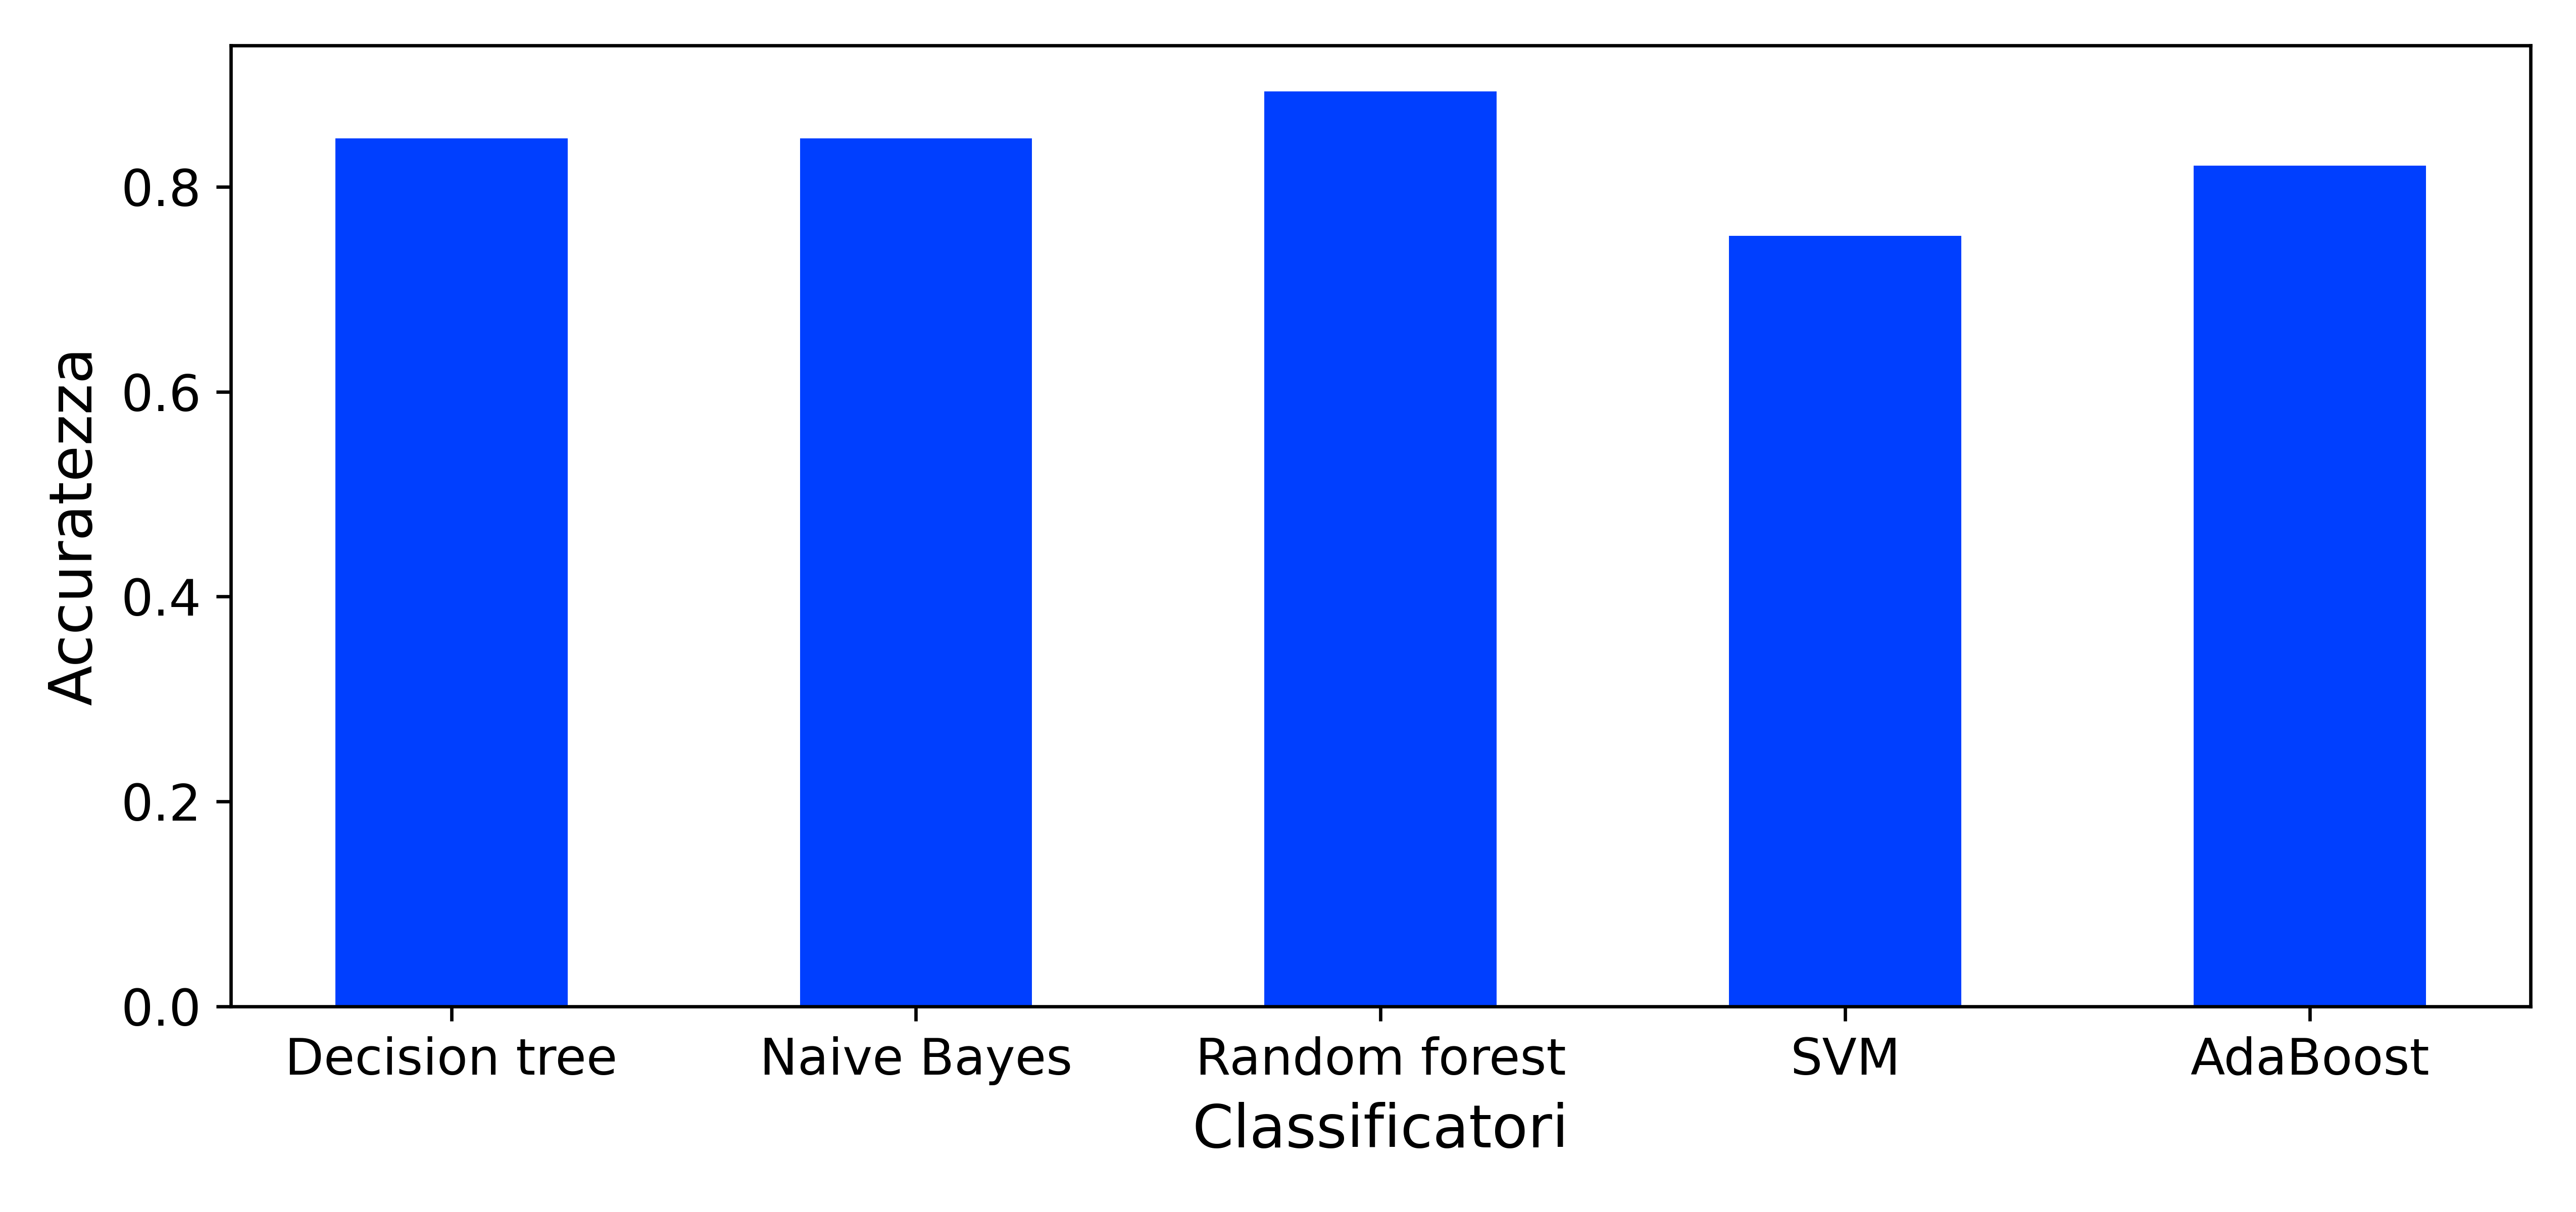
\includegraphics[scale=0.7]{../figure/Accuracy.png}
    \caption{Accuratezza classificatori}
    \label{fig:Accuracy}
\end{figure}

Successivamente ho preso in considerazione Precision e recall, quest'ultime mi danno la possibilità di analizzare più informazioni rispetto all'accuratezza, e inoltre mi permettono di avere una visione più completa delle prestazioni dei modelli implementati. Dalla tabella \ref{tab:PrecisionRecall} possiamo notare che in generale tutti i modelli hanno ottenuto risultati molto buoni per la predizione di file non vulnerabili, ma risultati poco precisi per la predizione di file vulnerabili, tra i diversi dati notiamo che il livello di precisione più alto raggiunto è stato di \numprint{0.34} per i file vulnerabili e \numprint{0.98} per i file non vulnerabili risultati ottenuti entrambi dal classificatore Random forest, mentre il livello di precisione più basso è stato ottenuto dal classificatore Naive Bayes con \numprint{0.08} per i file vulnerabili e \numprint{0.95} per i file non vulnerabili. \newline
\begin{table}[h]
    \centering
    \begin{tabular}{p{7cm}|r|r}
        \rowcolor{black}
        \textcolor{white}{\textbf{PREDIZIONE}} & \textcolor{white}{\textbf{PRECISION}} & \textcolor{white}{\textbf{RECALL}}\\  \multicolumn{3}{>{\columncolor{lightgray}}c}{\textbf{Decision tree}}\\
         File vulnerabili & \numprint{0.26} & \numprint{0.71}\\
         File non vulnerabili & \numprint{0.98} & \numprint{0.86}\\
         \multicolumn{3}{>{\columncolor{lightgray}}c}{\textbf{Naive Bayes}}\\
         File vulnerabili & \numprint{0.08} & \numprint{0.71}\\
         File non vulnerabili & \numprint{0.95} & \numprint{0.43}\\
         \multicolumn{3}{>{\columncolor{lightgray}}c}{\textbf{Random forest}}\\
         File vulnerabili & \numprint{0.34} & \numprint{0.71}\\
         File non vulnerabili & \numprint{0.98} & \numprint{0.91}\\
         \multicolumn{3}{>{\columncolor{lightgray}}c}{\textbf{SVM}}\\
         File vulnerabili & \numprint{0.14} & \numprint{0.53}\\
         File non vulnerabili & \numprint{0.96} & \numprint{0.77}\\
         \multicolumn{3}{>{\columncolor{lightgray}}c}{\textbf{AdaBoost}}\\
         File vulnerabili & \numprint{0.20} & \numprint{0.59}\\
         File non vulnerabili & \numprint{0.97} & \numprint{0.84} \\
    \end{tabular}
    \caption{Precision e Recall}
    \label{tab:PrecisionRecall}
\end{table}

Se guardiamo le prestazioni in termini di recall dei diversi modelli notiamo che il livello più alto per i file vulnerabili è di \numprint{0.71} ottenuto da tre classificatori diversi, mentre per i file non vulnerabili il risultato migliore è stato ottenuto dal Random forest con un livello di \numprint{0.91}, i risultati più bassi invece per i file vulnerabili sono stati registrati da SVM con \numprint{0.53}, mentre per i file non vulnerabili il livello più basso è stato di \numprint{0.43} ottenuto da Naive Bayes.
Attraverso la tabella \ref{tab:PrecisionRecall} è anche possibile notare le differenze in termini prestazionali dei vari classificatori, in particolare notiamo che in generale il classificatore con risultati più precisi è stato il Random forest seguito dal Decision tree, mentre il classificatore con risultati peggiori è stato il Naive Bayes, il quale ha registrato gli esiti più bassi per la predizione di file vulnerabili, registrando un grado di precisione molto basso. \newline
Dalla figura \ref{fig:F-measure} notiamo i risultati ottenuti in termini di F-measure dai diversi classificatori, questa misura attraverso un unico valore di permette di avere una visione più sintetica dei diversi risultati ottenuti dai classificatori, da questa misura notiamo che il classificatore che ha registrato maggiori prestazioni è stato il Random forest con un valore pari a \numprint{0.46}, mentre i risultati peggiori sono stati ottenuti dal classificatore SVM con \numprint{0.22}.

\begin{figure}[h]
    \centering
    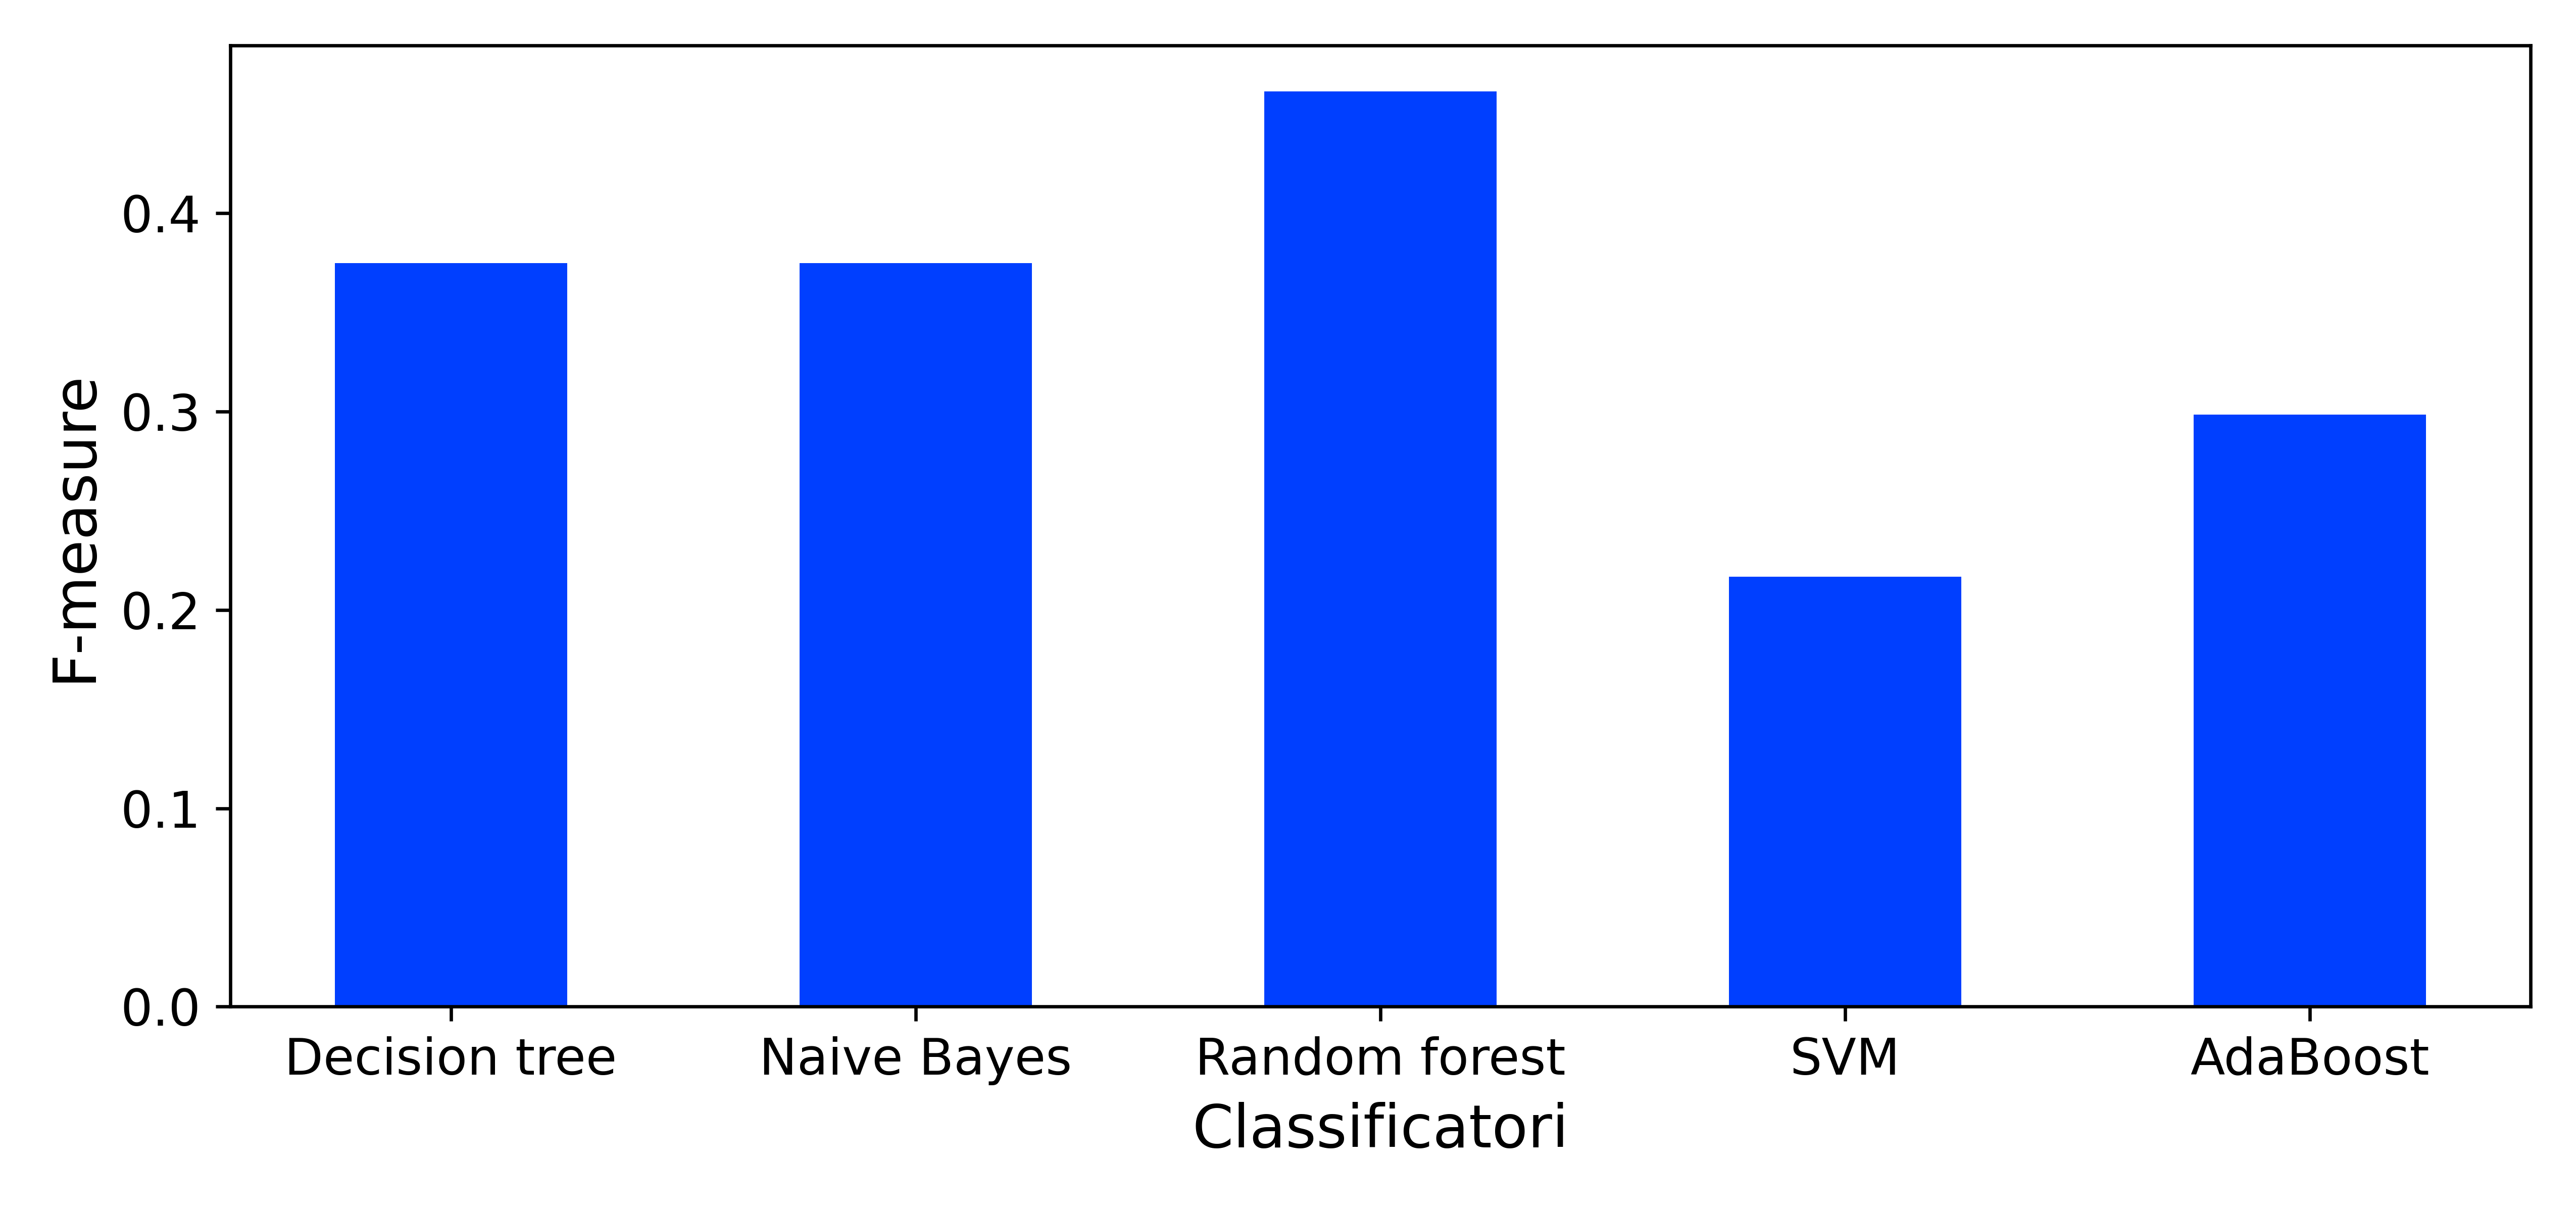
\includegraphics[scale=0.7]{../figure/F-measure.png}
    \caption{F-measure classificatori}
    \label{fig:F-measure}
\end{figure}


Confrontando le figure \ref{fig:Accuracy} e \ref{fig:F-measure} si possono notare risultati molto contrastanti tra F-measure e accuratezza, questa differenza è dovuta alla natura stessa del valore dell'accuratezza, quest'ultimo come descritto nel capitolo \ref{1cap:design} mette in relazione tutte le predizioni corrette con tutte le predizioni fatte dal modello in fase di validazione, è possibile comprendere questi esiti notando che il problema affrontato è fortemente sbilanciato ed i vari classificatori si comportano molto bene nella predizione dei file non vulnerabili, quindi durante la fase di validazione gran parte dei file presi in considerazione per la predizione sono file non vulnerabili, tutto ciò implica che il numero totale di predizioni esatte aumenta incrementando anche il livello di accuratezza.

Di particolare importanza durante la fase di validazione di un modello di predizione è visualizzare e analizzare la matrice di confusione ottenuta dalla validazione del modello, quest'ultima ha lo scopo di mettere in relazione tutte le predizioni che il modello ha eseguito con tutti i risultati reali del test selezionato per la validazione, nelle seguenti figure \ref{fig:CMNB}, \ref{fig:CMDT}, \ref{fig:CMRF}, \ref{fig:CMSVMe} e \ref{fig:CMAB}, sono stati riportati tutte le matrici di confusione di tutti i modelli implementati in questo studio. Leggendo questi dati possiamo notare che questi riflettono molto bene i dati analizzati precedentemente sopratutto valori di precision e recall analizzati nella tabella \ref{tab:PrecisionRecall}, inoltre ci permettono anche di comprendere il motivo di alcuni risultati ottenuti.
\begin{figure}[!ht]
\centering
    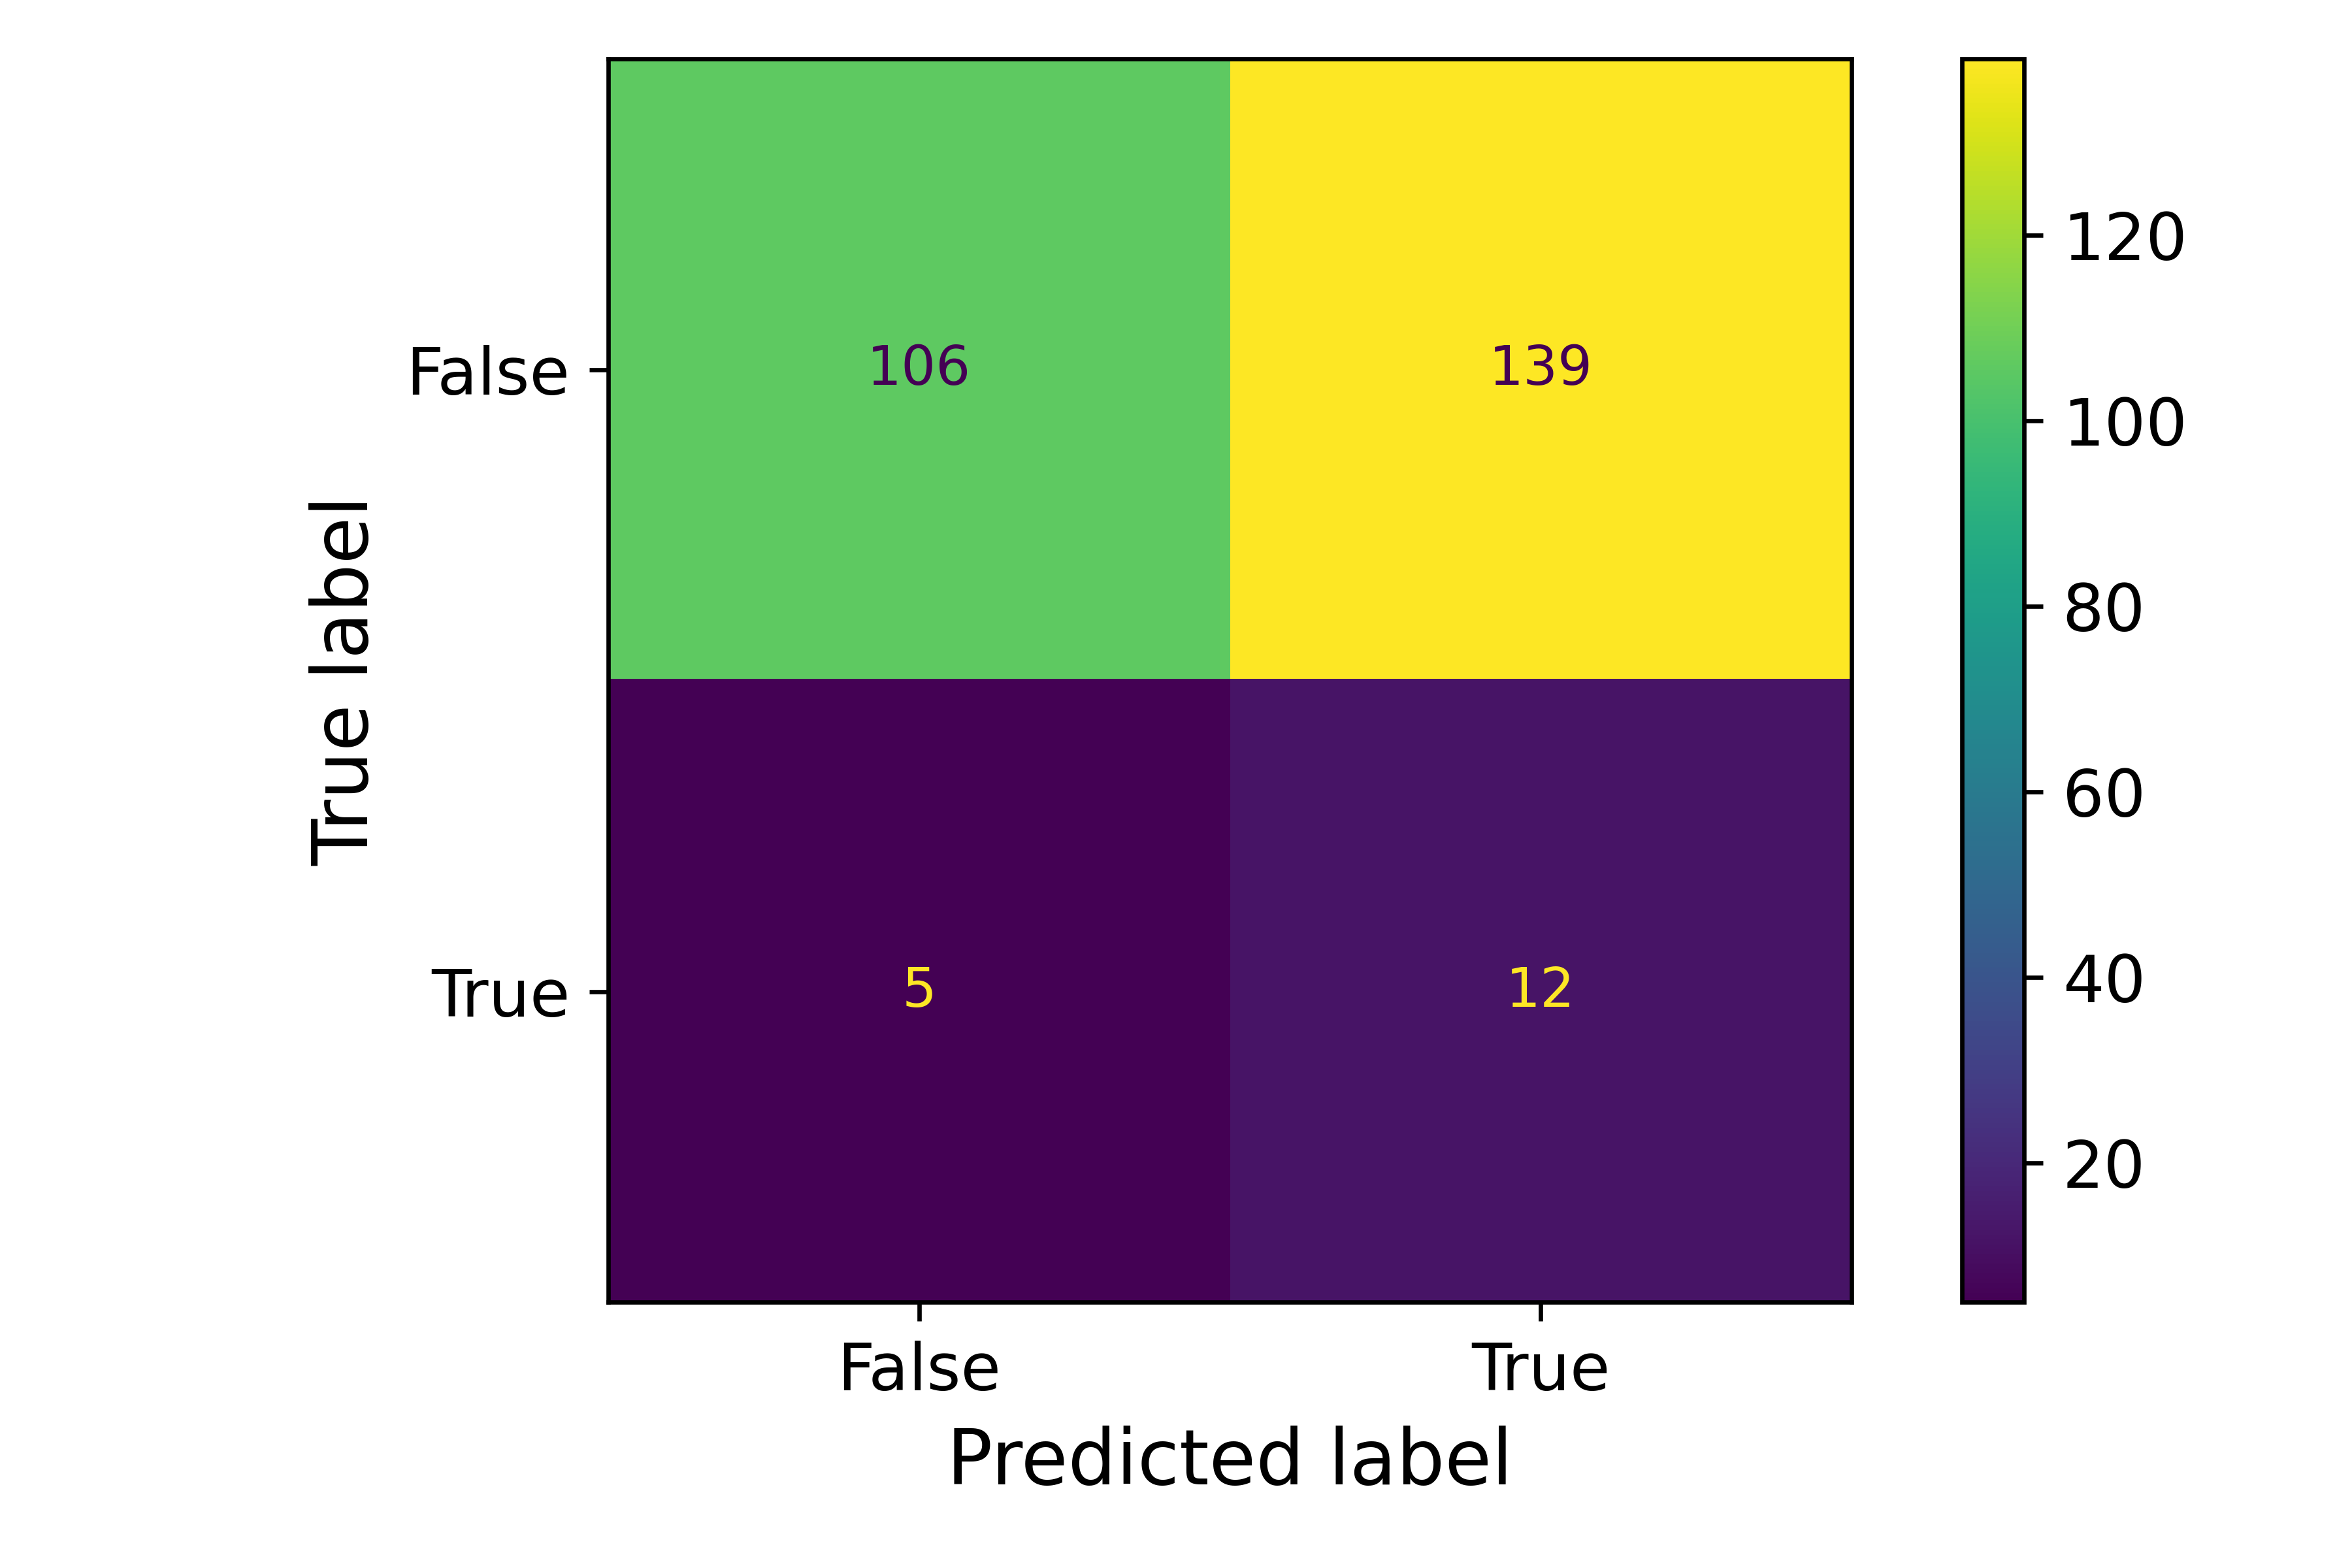
\includegraphics[scale=0.6]{../figure/NaiveBayesConfusionMatrix.png}
    \caption{Matrice di confusione Naive Bayes}
    \label{fig:CMNB}
\end{figure}
    
\begin{figure}[ht]
    \centering
    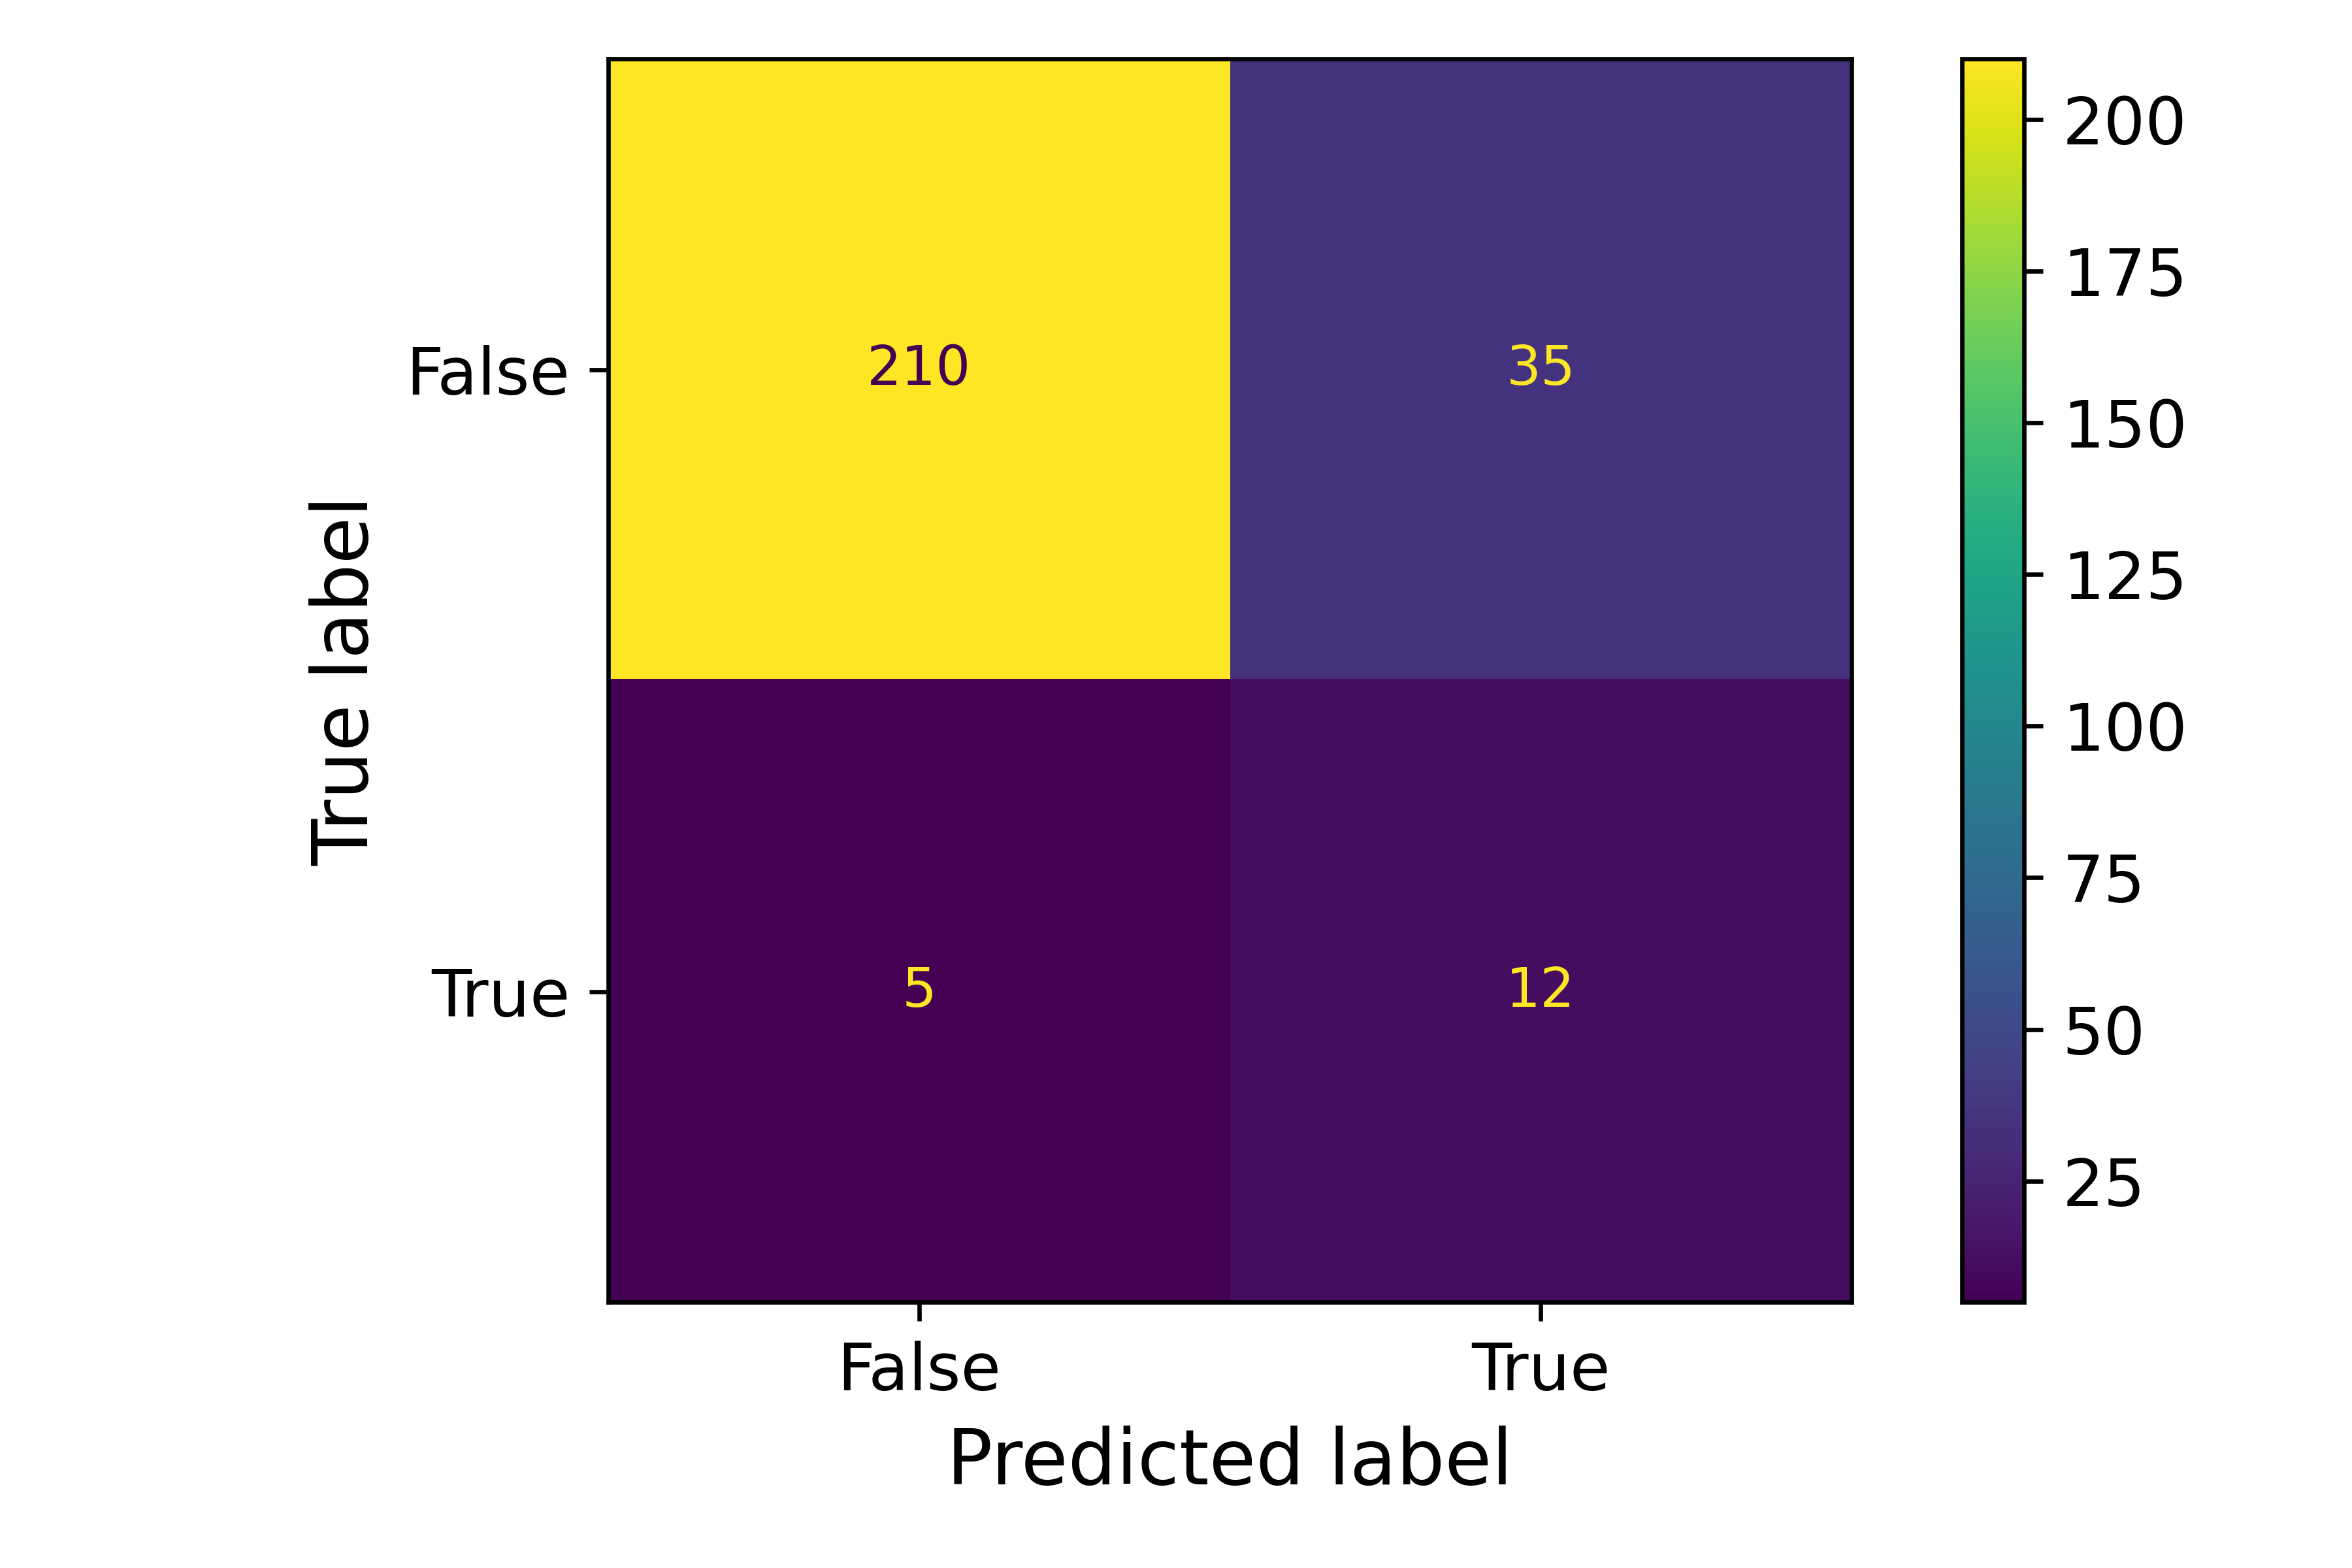
\includegraphics[scale=0.6]{../figure/DecisionTreeConfusionMatrix.png}
    \caption{Matrice di confusione Decision Tree}
    \label{fig:CMDT}
\end{figure}
Tra i dati più interessati emersi da questa analisi vediamo dalla matrice di confusione rappresentata dalla figura \ref{fig:CMNB} notiamo che il seguente classificatore in questo contesto ha una forte carenza per la predizione di file non vulnerabili, questo forte deficit influenza notevolmente il risultato di precision ciò spiega il motivo per cui questo modello ha riscontrato i livelli di precision più bassi di tutti i modelli implementati, questa forte carenza spiega anche il motivo per cui il seguente modello ha riscontrato il peggiore risultato di recall per la predizione di file non vulnerabili. Nonostante tutto notiamo che il classificatore Naive Bayes per i file vulnerabili ha predetto correttamente lo stesso numero di file dei classificatori che hanno raggiunto i risultati migliori e che sono Decision Tree \ref{fig:CMDT} e Random Forest \ref{fig:CMRF}. 
Il modello di predizione che invece ha registrato una bassissima capacità di predizione per file vulnerabili da come si evince dalla figura \ref{fig:CMSVMe} è stato il classificatore SVM con un numero di veri positivi migliore solo per una predizione nei confronti dei falsi positivi, nonostante ciò il classificatore ha ottenuto risultati migliori rispetto al classificatore Naive Bayes per la predizione dei file non vulnerabili, questo spiega il motivo per cui il SVM ha ottenuto risultati migliori in termini di precision.
Come detto in precedenza, analizzando i diversi classificatori notiamo che i risultati migliori ottenuti per la predizione di file vulnerabili sono analoghi per diversi classificatori, quindi il risultato migliore in termini di precision è legato al classificatore che ha una capacità predittiva maggiore per i file non vulnerabili, infatti come si nota dalla figura \ref{fig:CMRF} il classificatore Random forest ottiene i migliori risultati per la predizione di file non vulnerabili, ciò gli ha permesso di raggiungere i migliori risultati assoluti per il livello di precision.

\begin{figure}[]
    \centering
    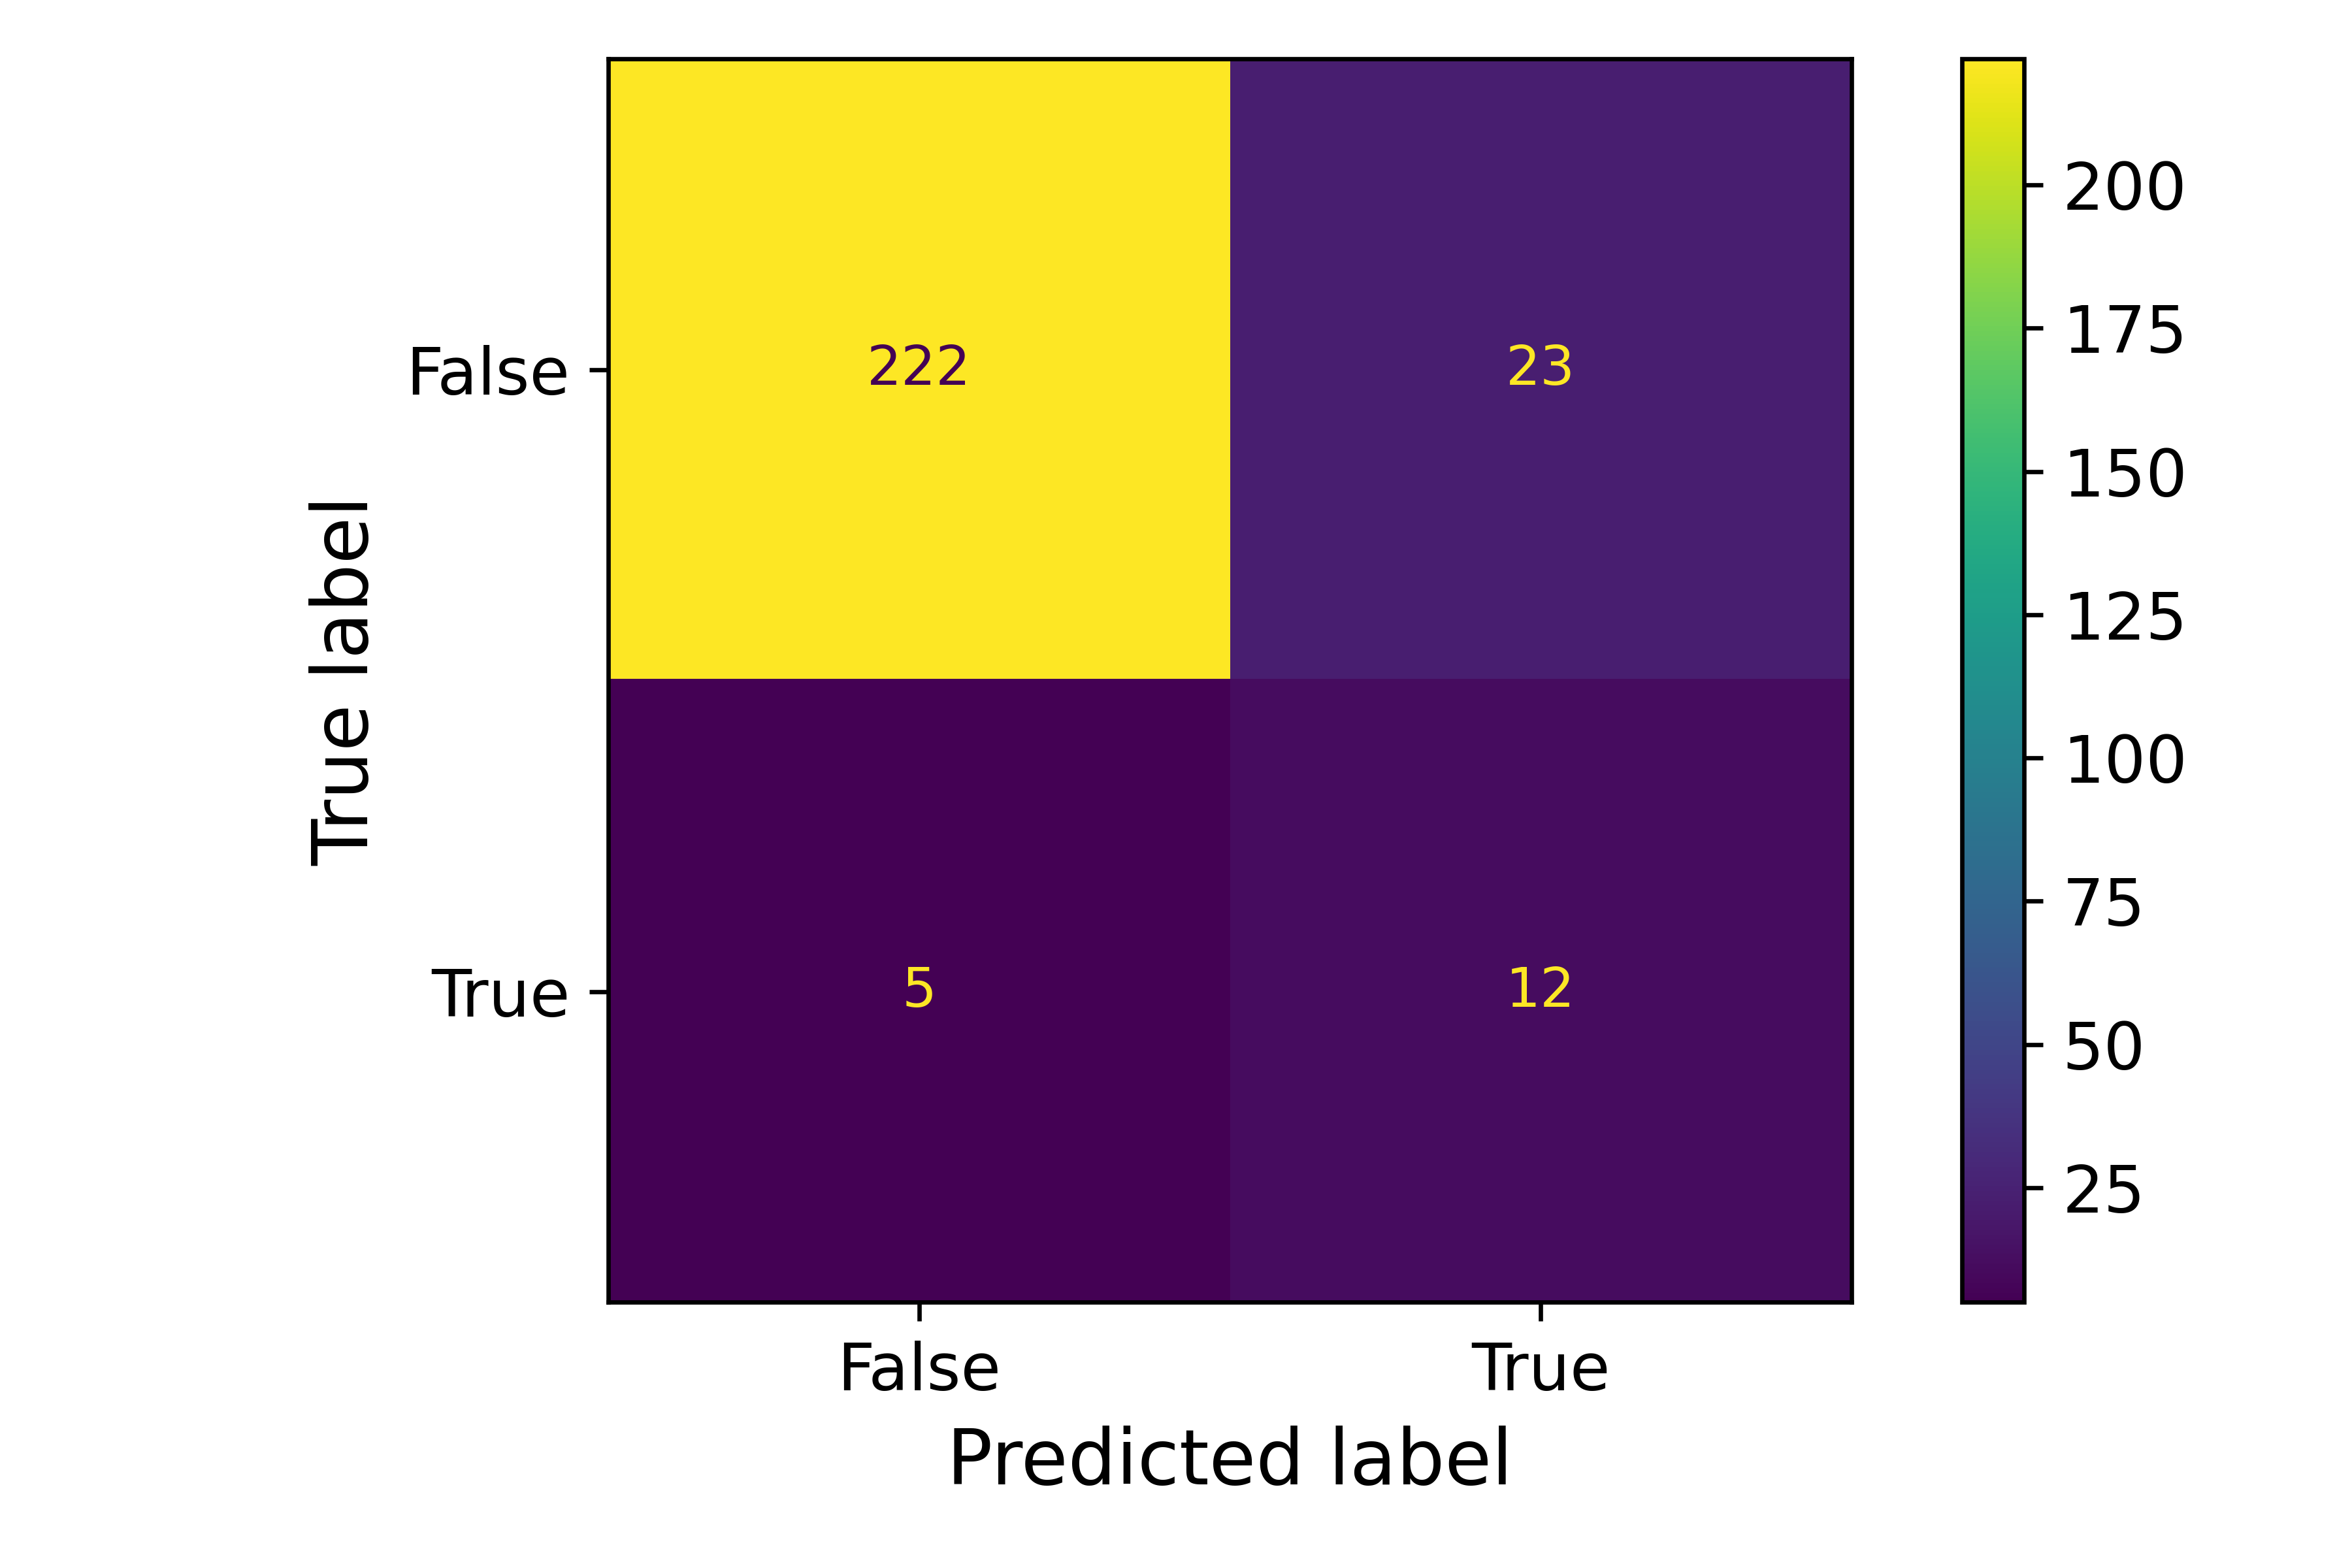
\includegraphics[scale=0.6]{../figure/RandomForestConfusionMatrix.png}
    \caption{Matrice di confusione Random forest}
    \label{fig:CMRF}
\end{figure}

\begin{figure}[!ht]
    \centering
    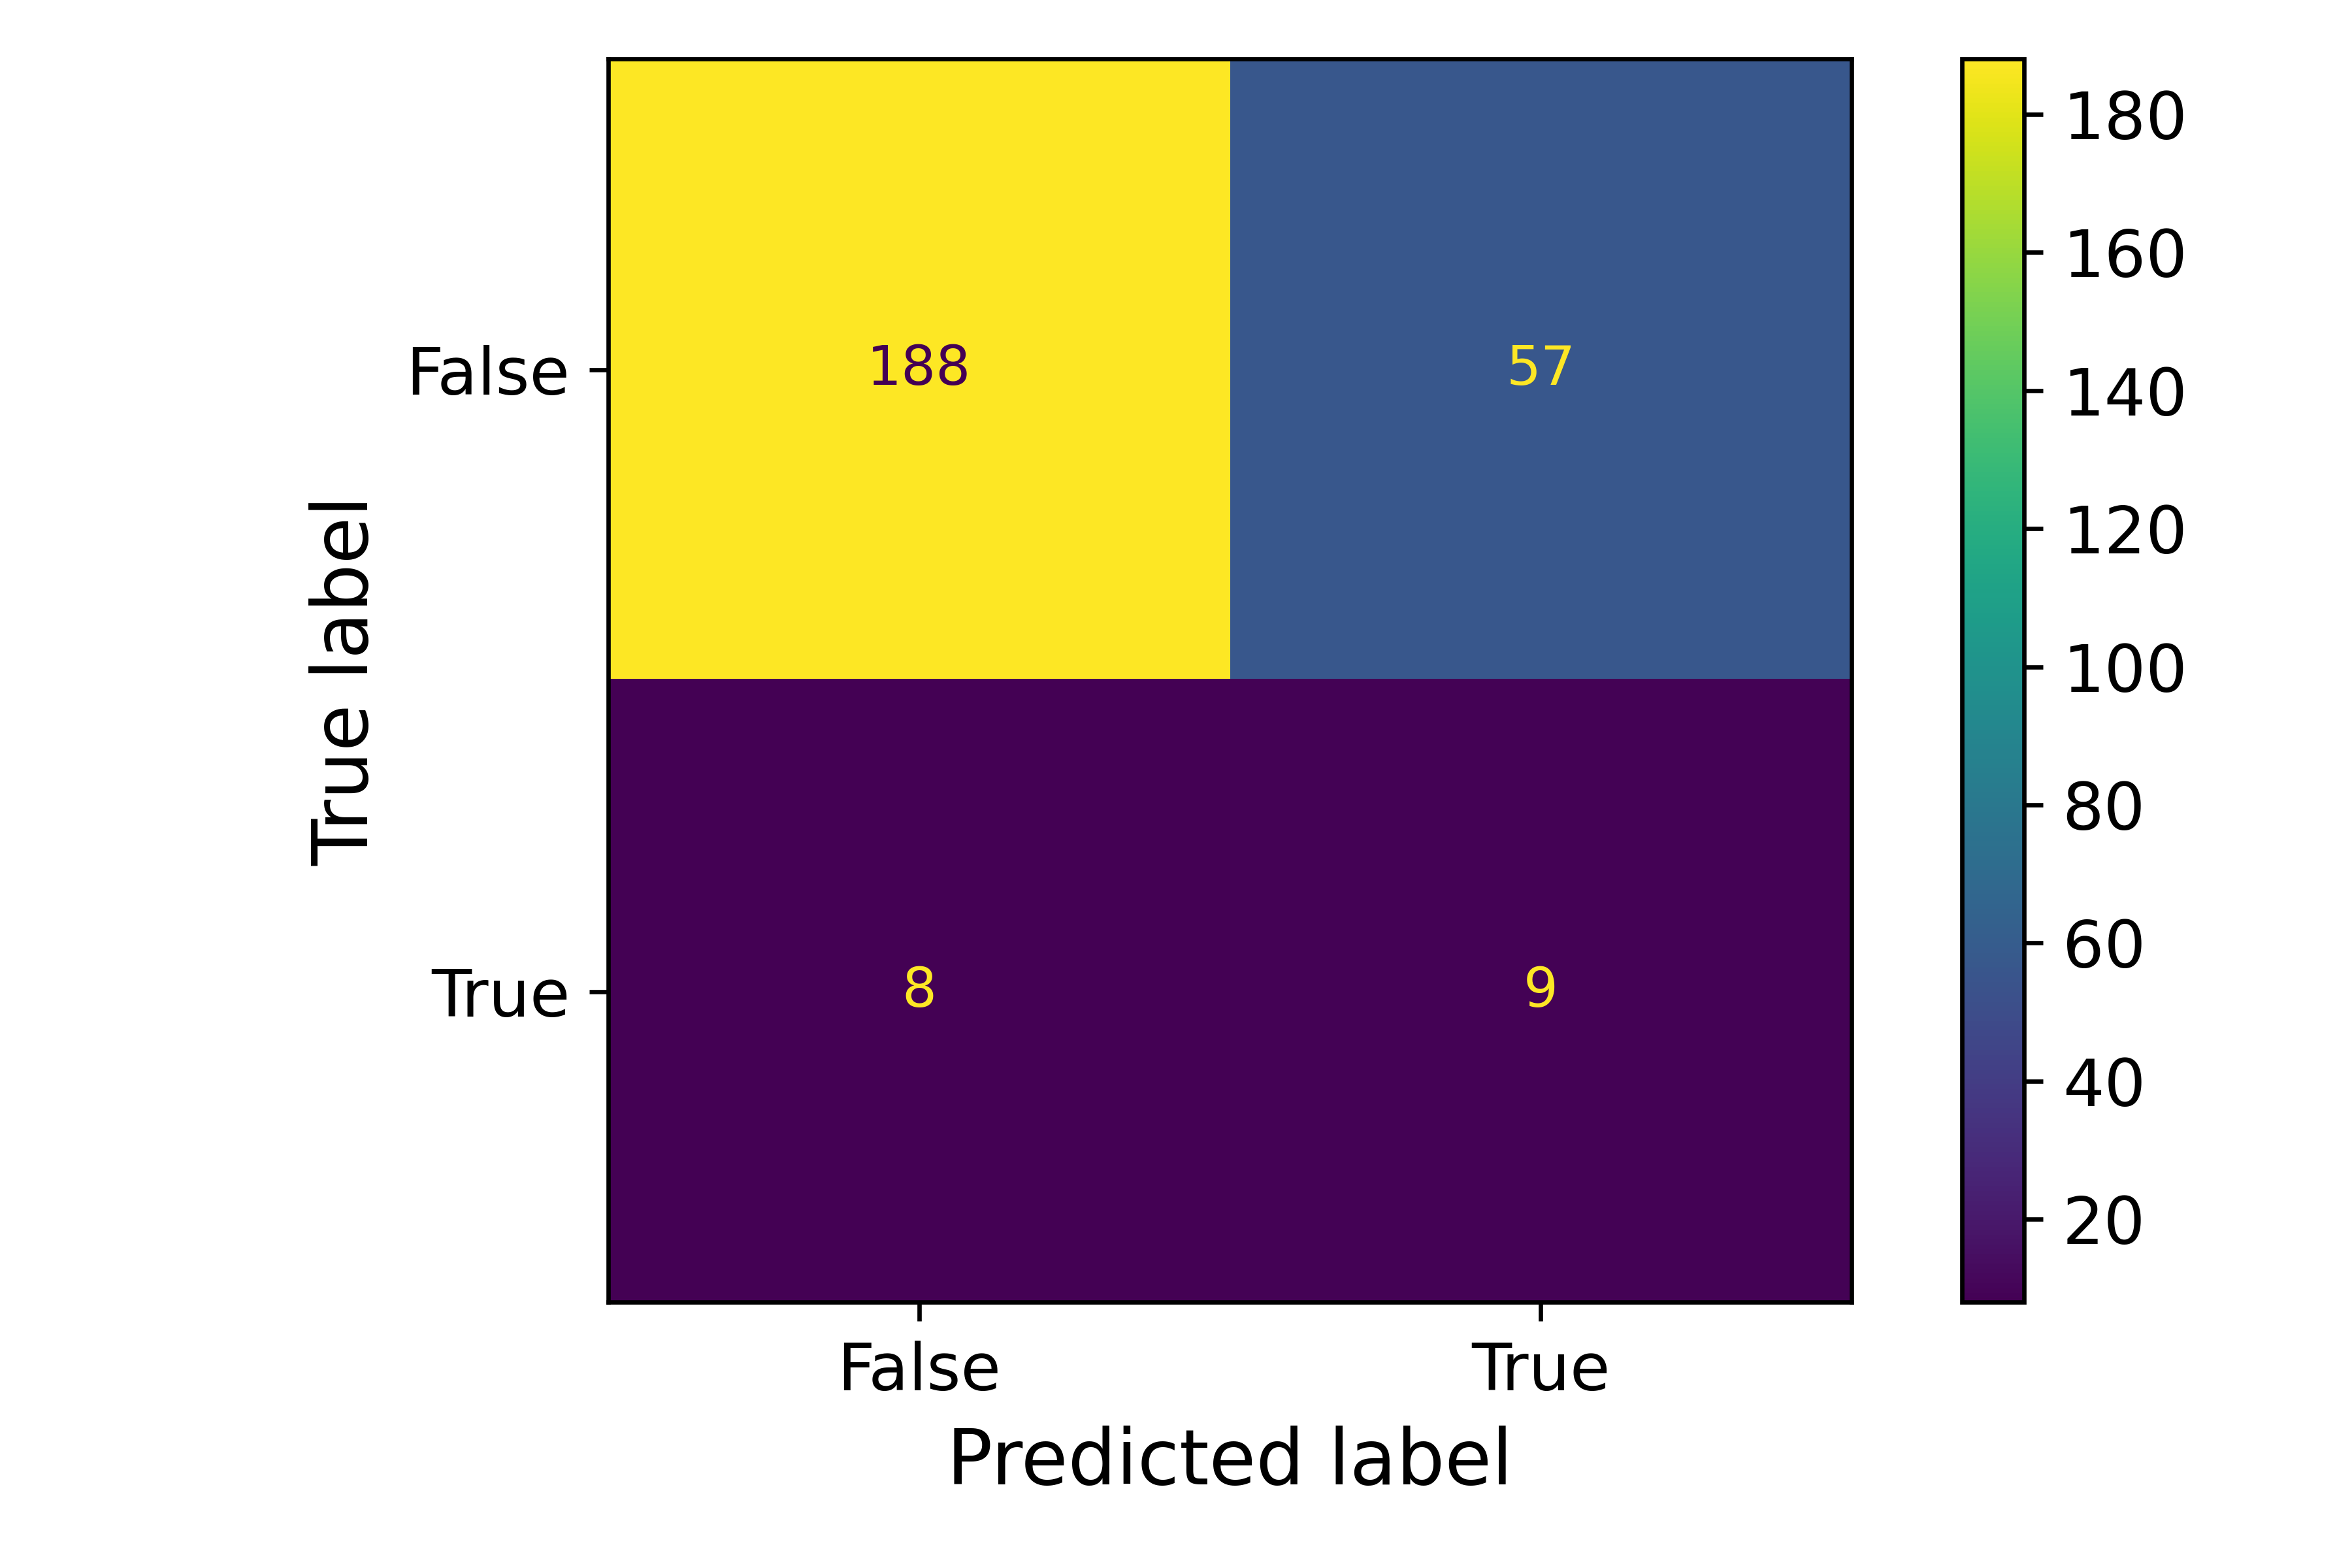
\includegraphics[scale=0.6]{../figure/SVMConfusionMatrix.png}
    \caption{Matrice di confusione SVM }
    \label{fig:CMSVMe}
\end{figure}

Dalle seguenti analisi possiamo osservare come i diversi classificatori operano ottenendo in alcuni casi risultati molto diversi tra loro. Nel ambito della predizione come si evince da questo studio e confermato da studi precedenti analizzati nel capitolo \ref{1cap:background} possiamo notare i classificatori più prestazionali per la predizione di vulnerabilità software sono quelli che prevedono la costruzione di uno o più alberi decisionali. Mentre il classificatore nel mio contesto che ha registrato performance più deludenti è stato il Naive Bayes, questo mostra come l'individuazione delle vulnerabilità software attraverso metriche software non è legato da fattori probabilistici. 

\begin{figure}[]
    \centering
    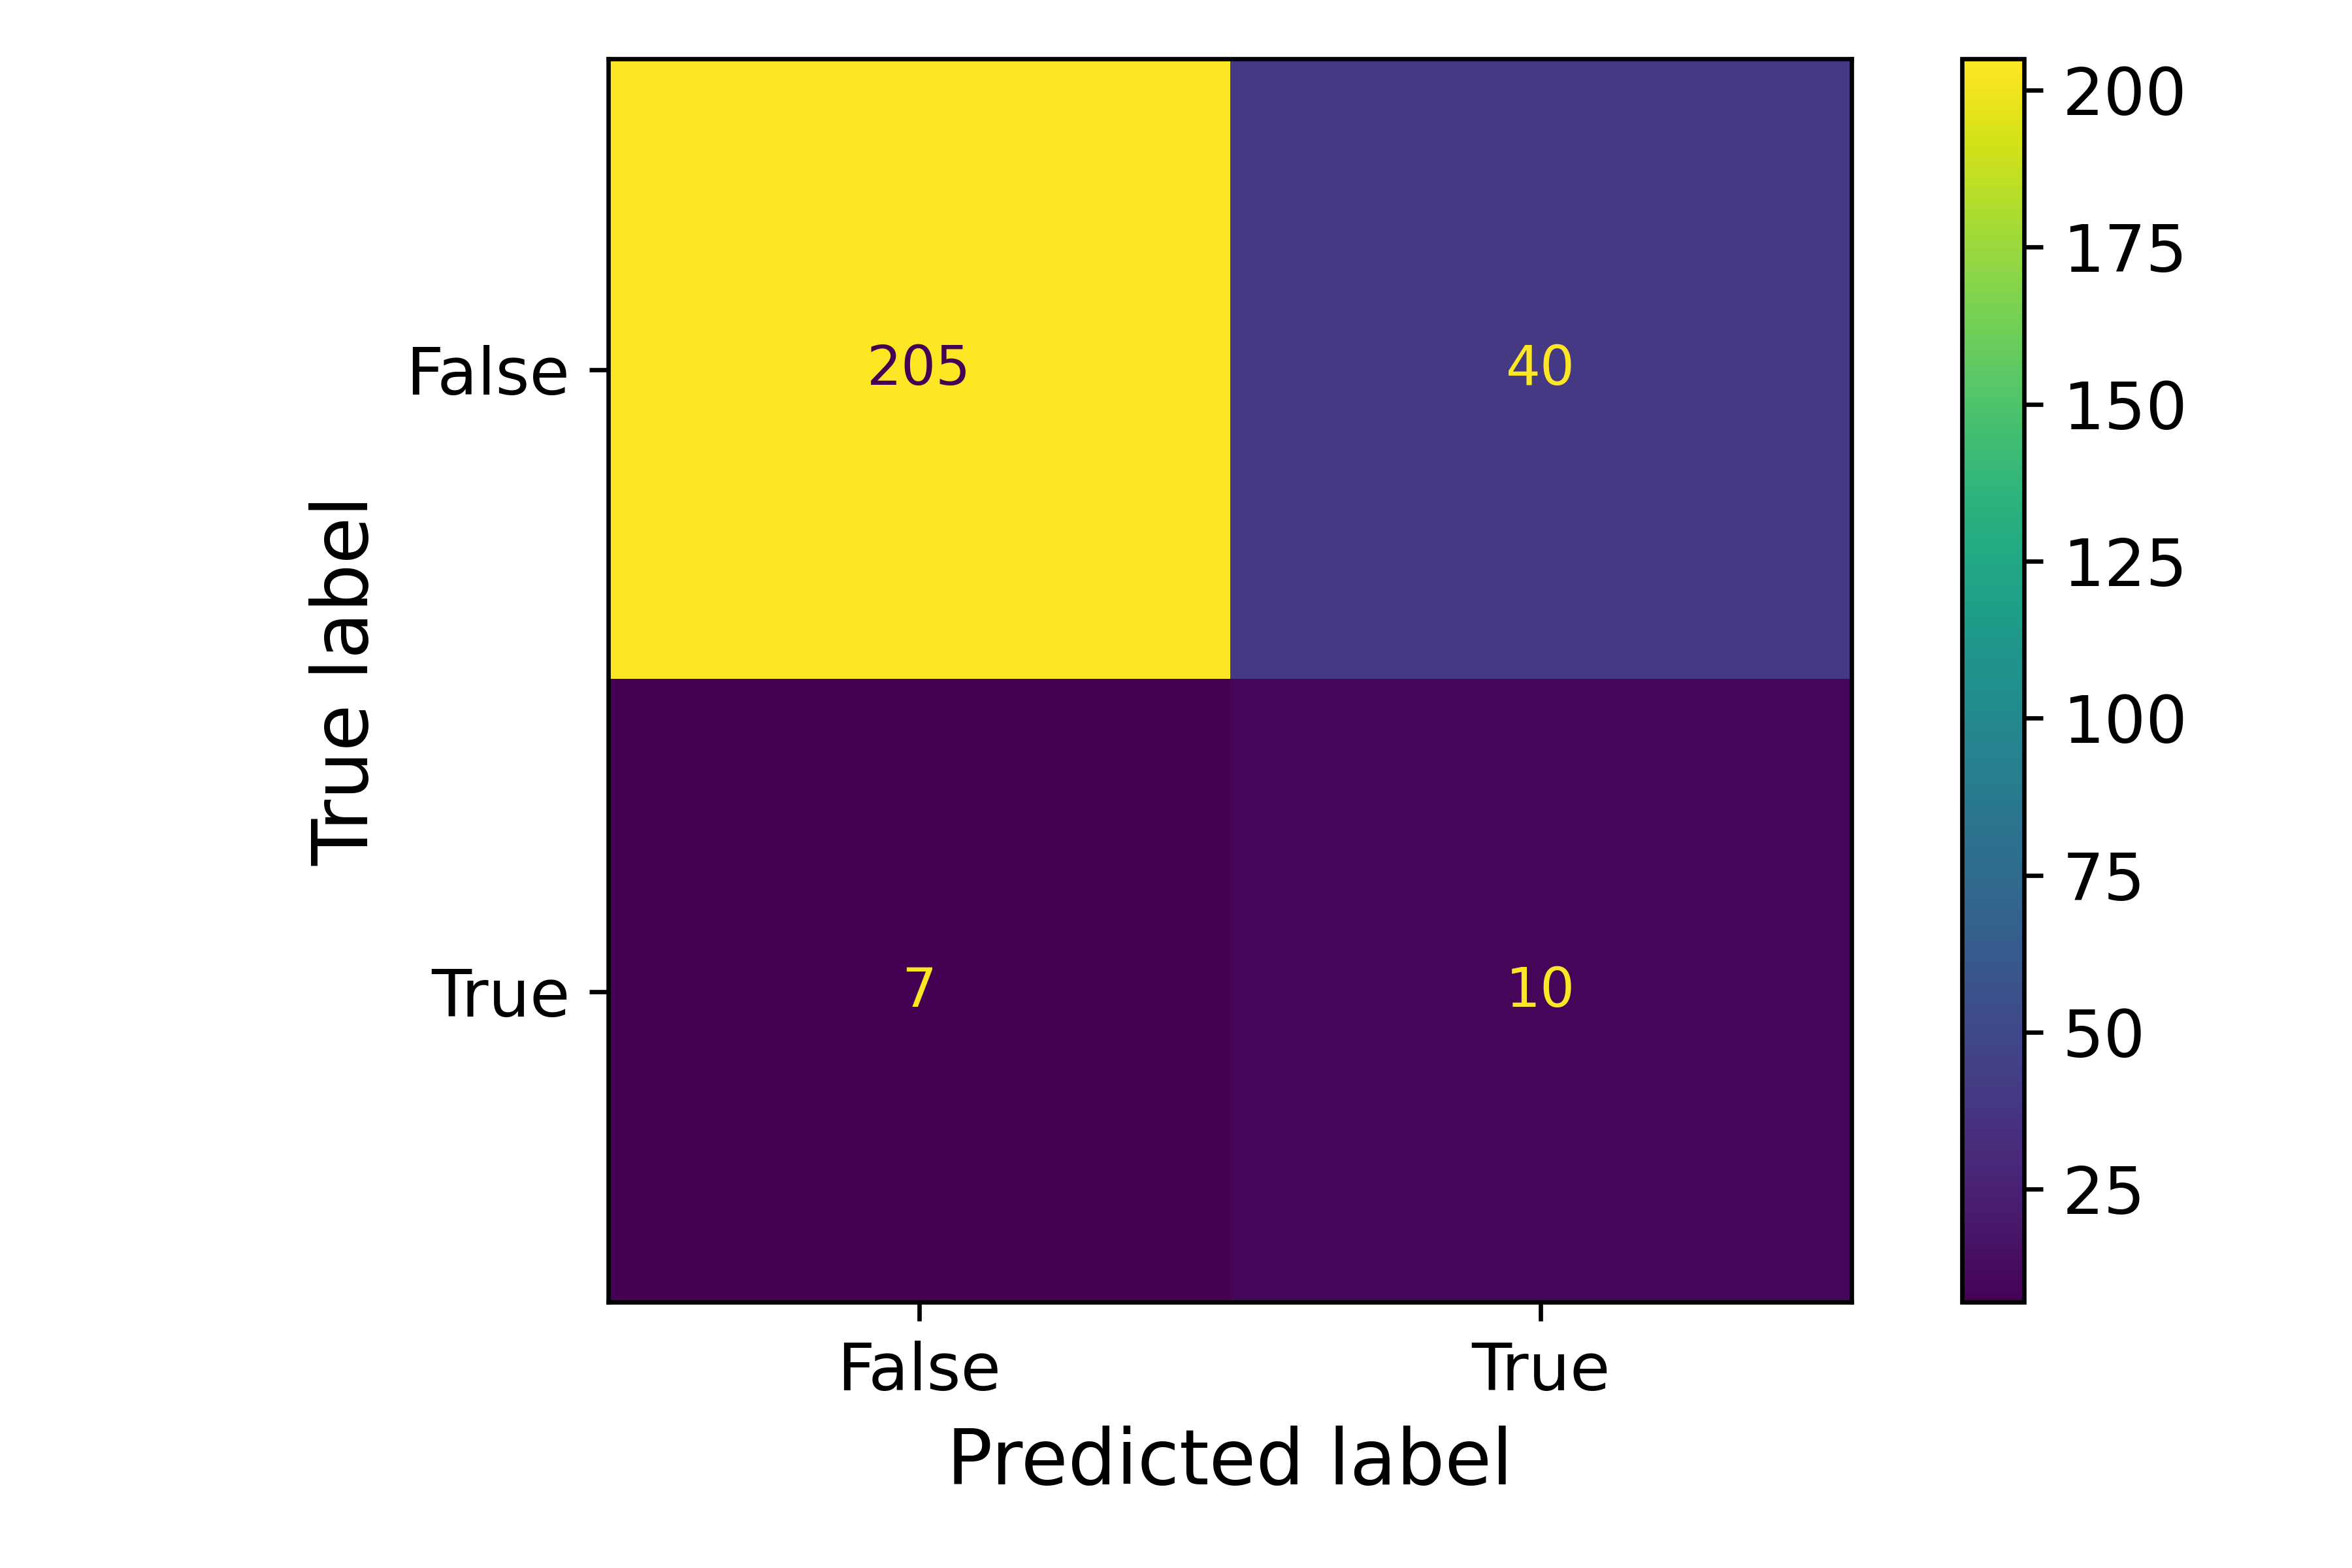
\includegraphics[scale=0.6]{../figure/AdaBoostConfusionMatrix.png}
    \caption{Matrice di confusione Ada Boost}
    \label{fig:CMAB}
\end{figure}


\newpage

\chapter{Conclusioni e sviluppi futuri} \label{1cap:conclusione}
% [titolo ridotto se non ci dovesse stare] {titolo completo}
%


In conclusione questo studio ha mostrato come e perché le vulnerabilità software coprono un ruolo di fondamentale importanza sul ciclo di vita del software e come queste possono influire notevolmente sulla vita degli utilizzatori, l'obiettivo principale di questo studio è stato di comprendere come le vulnerabilità possono essere individuate attraverso l'uso di VPM (modelli di predizione di vulnerabilità) analizzando come quest'ultimi lavorano e comprendendo il loro processo di implementazione. La parte più importante di questo lavoro è stata l'implementazione di un modello di predizione basato su machine learning che funzionasse sulla base di diverse metriche software, dalla costruzione del modello ho compreso come diverse metriche software possono lavorare insieme e quali di queste hanno un impatto maggiore, analizzando la loro correlazione con la presenza di vulnerabilità software. Dalla costruzione del modello ho potuto notare come i diversi classificatori lavorano e quali di questi hanno avuto un impatto migliore in termini di prestazioni per la predizione e il motivo legato questa differenza. \newline
Questo lavoro apre molte porte di sviluppo, essendo come punto di partenza per altri studi, uno dei lavori futuri più importanti potrebbe essere l'ottimizzazione del modello in termini di correttezza delle predizioni, questa ottimizzazione potrebbe essere sviluppata attraverso l'uso diversi algoritmi di ottimizzazione e di ricerca. Un importante lavoro potrebbe essere l'implementazione di un prodotto software sul quale installare il modello di predizione e che renda l'utilizzo del modello più semplice e veloce, e fruibile su più dispositivi. Questo lavoro per varie vicissitudini ha compreso ed analizzato un numero ridotto di metriche software anche se ne esistono un numero molto più grande ed alcune di queste raccolgono informazioni molto interessanti e che possono avere un impatto maggiore sulla corretta predizione del modello, per cui uno dei lavori più importanti è l'analisi di altre metriche software, con complessità diverse tra loro. Un importante sviluppo potrebbe essere la costruzione di un nuovo dataset, sulla base di quello usato da questo studio, che comprende diversi progetti con diverse complessità, integrando anche progetti software legati ad altri linguaggi di programmazione, in modo tale da creare un modello di predizione più preciso e complesso, il quale operi in modo corretto su più tipologie di prodotti software.
%\part{Impatto ambientale}

\backmatter
\begin{titlepage}

\nonumber
\null \vspace {\stretch{1}}
	\begin{flushright}
%	\begin{verse}
\textit{"Ascolta quel che insegna la sapienza, cerca di capire la sua lezione. Ricerca la conoscenza e desidera la saggezza, come si desidera l’argento o si va in cerca di tesori"} (La Bibbia).\\[5mm]
%	\end{verse}
	\end{flushright}
	
\end{titlepage}

\bibliographystyle{ieeetr}
\bibliography{bibliografia}

\end{document}
